\documentclass[twocolumn]{article}

\usepackage{titling}
\usepackage[margin=3cm,bottom=4cm,top=4cm]{geometry}
\usepackage{enumitem}
\usepackage{amssymb}
\usepackage{amsmath}
\usepackage{booktabs}
\usepackage{amsthm}
\usepackage{graphicx}
\usepackage{array}

\newtheorem{definition}{Definition}[subsection]
\newtheorem{corollary}{Corollary}[subsection]
\newtheorem{theorem}{Theorem}[subsection]
\newtheorem{lemma}{Lemma}[subsection]


\newcommand{\ex}[1]{\textbf{Exercise} \thesubsection.#1\par}
\newcommand{\defn}{\text{def}\textsuperscript{\underline{\text{n}}}\text{ }}
\newcommand{\soln}{\text{sol}\textsuperscript{\underline{\text{n}}}\text{ }}
\newcommand{\Thm}{\text{Th}\textsuperscript{\underline{\text{m}}}\text{ }}
\newcommand{\Ex}[1]{\textbf{Exercise} \thesubsection.#1}


\begin{document}

\twocolumn[
  \begin{@twocolumnfalse}
    \tableofcontents
  \end{@twocolumnfalse}
]

\clearpage

\twocolumn[
  \begin{@twocolumnfalse}
    \section{The Real Numbers}
  \end{@twocolumnfalse}
]
\setcounter{subsection}{2}
\subsection{The Axiom of Completeness}

\ex{1}
\begin{enumerate}[label=(\alph*)]

    \item
    For some $z \in \mathbb{Z}_5$, if we choose $y = 5 - z \pmod 5$ then
    \begin{align*}
        z + y   &= (5 - z) + z \pmod 5 \\
                &= 0 \pmod 5 
    \end{align*}
    Hence $y$ is an additive identity of $z$.

    \item
    This can be done explitly. \\
    \begin{center}
        \begin{tabular}{cc}
            \toprule
            $z$ & $x$ \\
            \midrule
            1 & 1 \\
            2 & 3 \\
            3 & 2 \\
            4 & 4 \\
            \bottomrule
        \end{tabular}
    \end{center}

    For example, for $z = 4, x = 4$:
    \begin{align*}
        xz  &= 4 \times 4 \pmod 5 \\
            &= 16 \pmod 5 \\
            &= 1 \pmod 5
    \end{align*}

    \item
    For $\mathbb{Z}_4$, then the construction in (a) will always be valid for a additive
    inverse. Hence an additive inverse exists for $\mathbb{Z}_n \, \forall \, n \in \mathbb N$. 

    Finding a multiplictive inverse is not always possible for any $z \in \mathbb Z_4$. For
    instance, $z = 2$ does not have a multiplictive inverse since any number multiplied
    by two will be even. However, we require the product to be $4n+1$ for some $n \in \mathbb N$
    which is impossible since the product will always be even.

    Hence, we conjecture that $\exists$ a multiplitive inverse $\forall \, z \in \mathbb Z_n$
    given $n$ is prime so that no element of $\mathbb Z_n$ shares a factor with n i.e. the greatest
    common divisor between any element of the set and n is 1.
    
\end{enumerate}

\ex{2}
\begin{enumerate}[label=(\alph*)]
    \item 
    \begin{definition}
        A real number $i$ is a greatest lower bound for a set $A \subseteq \mathbb{R}$ if it meets the following criteria:
        \begin{enumerate}[label=(\roman*)]
            \item $i$ is a lower bound for $A$.
            \item If $b$ is any lower bound for $A$, then $b \leq i $.
        \end{enumerate}
    \end{definition}

    \item
    \begin{lemma}
        Assume $i \in \mathbb{R}$ is a lower bound on a set $A \subseteq \mathbb{R}$. 
        Then $i = \inf A$ if and only if $\forall \, \varepsilon > 0 \, \exists \, a \in A $
        s.t. $i + \varepsilon > a$.  
    \end{lemma}

    \begin{proof}
        ($\Rightarrow$) Suppose $i = \inf A$, then $\forall \, \epsilon > 0 $ $ i+\varepsilon > i$
        but $i+\varepsilon$ cannot be a greater lower bound so there must exist $a \in A$ s.t. $i+\varepsilon > a$.

        ($\Leftarrow$) Suppose for some $i \in \mathbb{R}$ $i+\varepsilon > a$ for some $a \in A $ for arbitrary $ \varepsilon > 0$ then:
        \begin{enumerate}[label=(\roman*)]
            \item $i$ is a lower bound by assumption.
            \item Suppose $i \neq b = \inf A$ with $b>i$, then $b = i + \varepsilon$ for 
            $\varepsilon = |b - i|$ but $b =  i + \varepsilon > a$ for some $a \in A$ so
            we have reached a contradition since we assumed $b$ is a lower bound on A.
            Hence, $i$ is indeed the greatest lower bound.
        \end{enumerate}
    \end{proof}
\end{enumerate}

\ex{3}
\begin{enumerate}[label=(\alph*)]
    \item 
    \begin{proof}
        \begin{enumerate}[label=(\roman*)]
            \item 
            Suppose $\inf A$ is not an upper bound on B so $\exists$ $b \in B$ s.t. $\inf A \leq b$ but $b$ is a lower bound on $A$ so
            \begin{equation*}
                \inf A < b \leq a \, \forall a \in  A
            \end{equation*}
            This is a contradition since this would imply $b$ is a greater lower
            bound on A so we conclude $\inf A$ is indeed an upper bound on B.

            \item 
            A lower bound on $A$ is given by $\inf A - \varepsilon$ for any $\varepsilon > 0$ so $\inf A - \varepsilon \in B \forall \varepsilon > 0$. 
            But this would imply
            \begin{equation*}
                \inf A - \varepsilon < \inf A - \varepsilon/2 = b \in B
            \end{equation*}
            for any $\varepsilon >0$ which implies that $\inf A$ is a least upper bound for $B$.

            Alternatively, $\inf A$ is a lower bound on $A$ then $\inf A \in B$.
            So since $\inf A$ is an upper bound within $B$ then $\inf A$ is a maximum of $B$. If a maximum exists then $\sup B = \max B = \inf A$.
        \end{enumerate}
        Hence $\sup B = \inf A$.

        \item
        For set $A$ define set $-A = \{-a : a \in  A \}$. It is clear that $-A$ is bounded so we only need to prove
        \begin{equation*}
            -\sup(-A) = \inf A
        \end{equation*}
    \end{proof}
\end{enumerate}

\ex{4}
\begin{proof}
    If $B \subseteq A$ then $\forall b\in B \, \exists a \in  A$ s.t. $a \geq b$, this implies
    \begin{equation*}
        \sup A \geq a \geq \sup B
    \end{equation*}
\end{proof}

\ex{5}
\begin{enumerate}[label=(\alph*)]
    \item 
    \begin{proof}
        \begin{enumerate}[label=(\roman*)]
            \item 
            By \defn, $\forall a \in A \, \sup A \geq a$. 
            Adding $c$ to both sides we get $\forall a \in A \, c + \sup A \geq c + a $. Hence, $c + \sup{A}$ is an upper bound on $c+A$.

            \item 
            Now for arbitrary $\varepsilon > 0$, $\sup A - \varepsilon < a$ for some $a \in A$. This implies, $c + \sup A - \varepsilon < c + a \in c + A$ for some $a \in A$.
        \end{enumerate}
        Hence, $\sup{c+A} = c + \sup A$.
    \end{proof}

    \item
    \begin{proof}
        \begin{enumerate}[label=(\roman*)]
            \item 
            By \defn, $\forall a \in A \, \sup A \geq a$. 
            Multiplying by $c$ on both sides we get $\forall a \in A \, c \sup A \geq c a $. Hence, $c \sup{A}$ is an upper bound on $c A$.

            \item 
            Now for arbitrary $\varepsilon > 0$, $\sup A - \varepsilon < a$ for some $a \in A$. This implies, $c \sup A - \varepsilon < c a \in c A$ for some $a \in A$.

        \end{enumerate}
    \end{proof}

    \item 
    We postulate $\sup{cA} = -c \inf A$. This can be easily seen by imagining the sequence of maniplations from $A \rightarrow cA \rightarrow -cA$ and 
    observe how the up changes.
\end{enumerate}

\ex{6}
\begin{enumerate}[label=(\alph*)]
    \item $3$
    \item $1$
    \item $1/2$
    \item $9$
\end{enumerate}

\ex{7}
\begin{proof}
    Since is an upper bound by assumption, we only need to check that
    a is the least upepr bound. However, this is trivial since for arbitrary $\varepsilon > 0$ $a - \varepsilon < a \in A$ so $a = \sup A$.
\end{proof}

\ex{8}
\begin{proof}
    Let $\varepsilon = (\sup A + \sup B) / 2$. So
    \begin{equation*}
        \sup A < \sup B - \varepsilon < b
    \end{equation*}
    for some $b \in B$. So $b \in  B$ is an upper bound for $A$. 
\end{proof}

\ex{9}
\begin{enumerate}[label=(\alph*)]
    \item True
    
    \item 
    False, consider set 
    \begin{equation*}
        A = \left\{ L - \frac{1}{n} : n \in \mathbb{N} \right\}
    \end{equation*}
    where $\sup A = L$.
    
    \item 
    False, consider sets
    \begin{align*}
        A &= \left\{ L - \frac{1}{n} : n \in \mathbb{N} \right\} \\
        B &= \left\{ L + \frac{1}{n} : n \in \mathbb{N} \right\}
    \end{align*}
    However, $\inf B = \sup A = L$.

    \item True

    \item 
    False, consider sets
    \begin{align*}
        A &= \left\{ 1 - \frac{1}{n} : n \in \mathbb{N} \text{ and } n \text{ is even} \right\} \\
        B &= \left\{ 1 - \frac{1}{n} : n \in \mathbb{N} \text{ and } n \text{ is odd} \right\}
    \end{align*}
    Then, $\sup A = 1 \leq \sup B = 1$ but $\nexists \, b \in B$ that is an upper bound for $A$.

    This statement can be contradited more easily by noting that the 
    statement is false for two indentical sets with the supremum not in 
    the set. The above example demonstrates this statement is
    false for disjoint sets also.
\end{enumerate}
    

\clearpage
\subsection{Consequences of Completeness}

\ex{1}
\begin{theorem}
    For every two real numbers a and b
    with $a<b$, there exists a rational number r satisfying $a<r<b$.
\end{theorem}
\begin{proof}
    We consider two cases:
    \begin{itemize}
        \item $a < 0, b > 0$:
        By \Thm 1.4.3 $\exists$ $r$ s.t.
        \begin{equation*}
            a < 0 \leq r < b
        \end{equation*}

        \item $a<0, b \leq 0$:
        By \Thm 1.4.3 $\exists$ $r$ s.t. $-b < r < -a$ 
        $\Rightarrow a < -r < b$.
    \end{itemize}
\end{proof}

\ex{2}
\begin{enumerate}[label=(\alph*)]
    \item 
    \begin{proof}
        Let $p/q, r/s \in \mathbb{Q}$ with $p, q, r, s \in \mathbb{Z}$, then
        \begin{align*}
            \frac{p}{q} + \frac{r}{s} = \frac{ps+rq}{qs} \in \mathbb{Q}
        \end{align*}

        Similarly,
        \begin{align*}
            \frac{p}{q} \frac{r}{s} = \frac{pq}{rs} \in \mathbb{Q}
        \end{align*}
    \end{proof}

    \item 
    \begin{proof}
        We proceed by contradiction:
        Suppose $p,q,r,s \in \mathbb{Z}$ with $a=p/q$, then
        \begin{align*}
            at = \frac{p}{q}t   &= \frac{r}{s} \\
                  \Rightarrow t &= \frac{rq}{sp} \in \mathbb{Q} 
        \end{align*}
    \end{proof}
    However, $t$ is irrational.

    \item 
    $\mathbb{I}$ is not closed under addition or multiplication.
    For instance, consider examples
    \begin{align*}
        - \sqrt 2 + \sqrt 2 = 0 \in \mathbb{Q} \\
        \sqrt 2 \sqrt 2 = 2 \in \mathbb{Q} 
    \end{align*}
\end{enumerate}

\ex{3}
\begin{corollary}
    Given any two real numbers $a<b$, there exists an irrational
    number $t$ satisfying $a<t<b$.
\end{corollary}
\begin{proof}
    Using \Thm 1.4.3 $\exists \, r \in \mathbb{Q}$ s.t. 
    \begin{equation*}
        a - \sqrt 2 < r < b - \sqrt 2 
    \end{equation*}
    given $a < b$. However, if we add $\sqrt 2$ this implies 
    \begin{equation*}
        a < r + \sqrt 2 < b
    \end{equation*}
    Using \Ex{2} we can conclude that $t = r + \sqrt 2 \in \mathbb{I}$.
\end{proof}

\ex{4}
\begin{proof}
    Let $A = \inf \{ 1/n: n \in \mathbb{N} \}$
    \begin{enumerate}[label=(\alph*)]
        \item 
        Since $1/n \neq 0$ for any $n \in  \mathbb{N}$ then 0
        is indeed a lower bound for A.

        \item 
        By the Archimedean Property of $\mathbb{R}$ for any
        $\varepsilon > 0 \, \exists n \in \mathbb{N}$ s.t.
        \begin{equation*}
            0 + \varepsilon = \varepsilon > 1/n \in A
        \end{equation*}
    \end{enumerate}
    Hence $\inf A = 0$.
\end{proof}

\ex{5}
\begin{proof}
    We proceed by contradiction, suppose $\exists x \in \bigcap_{n=1}^{\infty}$,
    However, by the Archimedean Property $ \exists m \in \mathbb{N}$ s.t.
    $x > 1/n$ so $x \notin (0,1/m) \Rightarrow x  \notin \bigcap_{n=1}^{\infty} (0,1/n)$
\end{proof}

\ex{6}
\begin{enumerate}[label=(\alph*)]
    \item 
    Continuing on from the proof of \Thm 1.4.5:
    By the Archimedean Property $\exists$ $n_0 \in \mathbb{N}$ s.t. 
    $1 / n_0 < \frac{\alpha^2+2}{2\alpha} $ which implies
    \begin{equation*}
        \left( \alpha - \frac{1}{n_0} \right) > \alpha^2 - \frac{2\alpha}{n_0} > 2
    \end{equation*}
    But we assumed $\alpha$ is a least upper bound so we have reached a 
    contradition. Hence, $\alpha^2 = 2 \Rightarrow \alpha=\sqrt 2$.

    \item
    We only need to repeat the proof given in \Thm 1.4.5 using the set
    \begin{align*}
        S = \{ s\in \mathbb{R}: s^2 < b \}
    \end{align*}
    We would conclude $\sup S = \sqrt b$.
\end{enumerate}

\ex{7}
\begin{theorem}
    If $A \subseteq B$ and $B$ is countable, then $A$ is either countable,
    finite, or empty.
\end{theorem}
\begin{proof}
    We proceed by induction: We will induct on the domain of $g: \mathbb{N} \rightarrow A$.
    
    \begin{itemize}
        \item 
        Base case ($m = 1$):
        Let $T_1 = \{ n_1 \in \mathbb{N} : f(n) \in A \}$. Let $n_1 = \min T_1$
        and $g(1) = f(n_1)$.

        \item 
        Inductive step: ($m > 1$): Let $T_{m+1} = T_m\\ n_m$. Let $n_{m+1} = \min T_{m+1}$
        and $g(n_{m+1}) = f(n_{m+1})$.
    \end{itemize}
    Clearly $g$ will be 1-1 and onto since $\text{dom} g$ and $\text{ran} g$ are 
    subsets of $\text{dom} f$ and $\text{ran} f$ respectively which is also 1-1 and onto.
    
    If $A$ is either empty or finite then the indcution stops at some $m$.
\end{proof}

\ex{8}
\begin{enumerate}[label=(\alph*)]
    \item 
   \begin{proof}
        Without loss of generality suppose $A_1, B_2$ are disjoint. We begin by
        assuming that both sets are infinite. Since $B_2 \subseteq A_2$ we proved
        in \Ex{7} that $B_2$ is countable so $\exists$ bijections
        \begin{align*}
            f &: A_2 \rightarrow \mathbb{R} \\
            g &: B_2 \rightarrow \mathbb{R}
        \end{align*}
        We define new function $h : \mathbb{N} \rightarrow A_1 \cup B_2$ by
        \begin{equation*}
            h(n) = \begin{cases} 
                f(\frac{n+1}{2}) & n \text{ odd} \\
                g(\frac{n}{2}) & n \text{ even}
            \end{cases}
        \end{equation*}
        $h$ simply returns the elements of $A_1$ and $B_2$ in alternating order.
        Since $h$ is 1-1 (since $A_1$ and $B_2$ are disjoint) and onto we can
        conclude $A_1 \cup B_2$ is countable. However since $A_1 \cup B_2 = A_1 \cup A_2$
        then the same conclusion follows for any two infinite countable sets.
        
        If $B_2$ is finite with $m$ elements then we simply define
        \begin{equation*}
            h(n) = \begin{cases} 
                g(n) & n \leq m \\
                f(n-m) & n > m
            \end{cases}
        \end{equation*}

        By induction this result can be generalized to an arbitrary number of sets
        since every induction step only involves the union of two countable sets
        which we have proven.
   \end{proof}

   \item
   We cannot induct on infinity, what case came before infinity?

   \item
   Let $f_m: \mathbb{N} \rightarrow A_m \, \forall m \in \mathbb{N}$ and 
   $A = \{ f_m \in m\in \mathbb{M} \}$.

   For each $m\in \mathbb{N}$, we could assign $A_m$ to the $m^{\text{th}}$ row
   of the grid and the $n^{\text{th}}$ element of $A_m$ to the $n^{\text{th}}$ 
   column. To that end, we define bijective function $k : \mathbb{N} \times \mathbb{N} \rightarrow A$ given by
   \begin{equation*}
        k(n,m) = f_n(m)
   \end{equation*}

   Next let $g: \mathbb{N} \times \mathbb{N} \rightarrow \mathbb{N}$ which 
   takes in a row and a column and returns the corresponding value in the 
   two-dimensional array in illustrated in the preblem. Hence $g$ is bijective 
   so $g^{-1}$ also exists and undoes the mapping.
   
   The composition of bijective functions is bijective so we can define
   $\ell : \mathbb{N} \rightarrow \bigcup_{n=1}^\infty A_n$ By
   \begin{equation*}
        \ell = k \circ g^{-1}
   \end{equation*}
   which would prove $\bigcup_{n=1}^\infty A_n$ is countable.
    
\end{enumerate}

\ex{9}
\begin{enumerate}[label=(\alph*)]
    \item 
    If $A \sim B$ then $\exists$ bijection $f: A\rightarrow B$. However, 
    the inverse of a bijection is a bijection so $f^{-1}$ exists and is bijective
    which implies $B\sim A$.

    \item
    The result follows trivially using the fact that the composition of 
    bijective functions is a bijection. That is, if $f:A \rightarrow B$ and 
    $g:B \rightarrow C$ then $h:A\rightarrow C$ is a bijection and implies $A \sim C$.
\end{enumerate}

\ex{10}
\clearpage


\twocolumn[
  \begin{@twocolumnfalse}
    \section{Sequences and Series}
  \end{@twocolumnfalse}
]
\setcounter{subsection}{1}
\subsection{The Limit of a Sequence}

\ex{1}
\begin{enumerate}[label=(\alph*)]
    \item 
    $\lim \frac{1}{6n^2+1} = 0$

    Scratchwork: We require that for some $\varepsilon > 0$
    \begin{align*}
        \frac{1}{6n^2+1} &< \varepsilon \\
        \Rightarrow n &> \sqrt{\frac{1}{6}\left( \frac{1}{\varepsilon} - 1 \right)}
    \end{align*}
    So we choose $N > \sqrt{\frac{1}{6}\left( \frac{1}{\varepsilon} - 1 \right)}$.

    \begin{proof}
        Let $\varepsilon>0$ be arbitrary. 
        For $n \geq N > \sqrt{\frac{1}{6}\left( \frac{1}{\varepsilon} - 1 \right)}$ where $n, N\in \mathbb N$
        then
        \begin{align*}
            \left| \frac{1}{6n^2+1}\right| &< \left| \frac{1}{6N^2+1}\right| \\
                                            &< \varepsilon
        \end{align*}
        
    \end{proof}

    \item 
    $\lim \frac{3n+1}{2n+5} = 3/2$

    \begin{proof}
        Let $\varepsilon>0$ be arbitrary. 
        For $n \geq N > \frac{1}{4}\left( \frac{13}{\varepsilon} - 10 \right)$ where $n, N\in \mathbb N$
        then
        \begin{align*}
            \left|  \frac{3n+1}{2n+5} - \frac{3}{2} \right| < \varepsilon
        \end{align*}
    \end{proof}

    \item
    $\lim \frac{2}{\sqrt{n+3}} = 0$

    \begin{proof}
        Let $\varepsilon>0$ be arbitrary. 
        For $n \geq N > \frac{4}{\varepsilon^2}-3$ where $n, N\in \mathbb N$
        then
        \begin{align*}
            \left|  \frac{2}{\sqrt{n+3}} \right| < \varepsilon
        \end{align*}
    \end{proof}
\end{enumerate}

\ex{2}
Consider this sequence which is vercongent but divergent
\begin{align*}
    (-1,1,-1,1,...)
\end{align*}
The defintion of vercongence is simply that the sequence be bounded above and 
below. The bound is called $\varepsilon$.

\ex{3}
\begin{enumerate}[label=(\alph*)]
    \item Find a college in the US with no students above seven feet.
    \item Find a college in the US where every professor has given a
    grade other than an A or B.
    \item Find a student at every US college which is below six feet.
\end{enumerate}

\ex{4}
The greatest distance between the largest and smallest terms of the sequence
 are $0$ and $1$ so for any $\varepsilon > 1$ then 
 \begin{align*}
    |a_n - 0| \leq 1 < \varepsilon
 \end{align*}
 for any $n \leq N = 1$ where $n, N \in \mathbb{N}$. Conversely, for $\varepsilon \leq 1$
 there exists no suitable response.

 \ex{5}
 \begin{enumerate}[label=(\alph*)]
    \item 
    Observe $a_n = 0$ for $n > 1$ so 
    \begin{align*}
        |a_n - 0| = 0 \quad \forall n \geq N > 1 
    \end{align*}
    So $(a_n) \rightarrow 0$.

    \item 
    Observe, for $n>10$ $10+n < 2n$ so the tail of the sequence is imply zeros so
    $N = 11$ is a suitable response to any $\varepsilon > 0$.
 \end{enumerate}

\ex{6}
\begin{enumerate}[label=(\alph*)]
    \item larger
    \item larger
\end{enumerate}

\ex{7}
\begin{enumerate}[label=(\alph*)]
    \item 
    \begin{definition}
        A sequence $(a_n)$ converges to infinity if for every 
        $\varepsilon > 0$, there exists $N \in \mathbb{N}$ s.t. 
        for all $n \geq N$ it follows $|a_n| > \varepsilon$.
    \end{definition}

    We now prove $(\sqrt n)$ converges to infinity.
    \begin{proof}
        Let $\varepsilon > 0$ be arbitrary, then
        \begin{align*}
            |\sqrt n | > \varepsilon \quad \forall n \geq \mathbb{N} > \varepsilon
        \end{align*}
    \end{proof}

    \item 
    This sequence does not converge to infinity since oscillates.
\end{enumerate}

\ex{8}
\begin{enumerate}[label=(\alph*)]
    \item frequently
    \item Eventually is stronger than frequently since eventually 
    $\Rightarrow $ frequently.

    \item
    \begin{definition}
        A sequence $(a_n)$ converges to a if, given any $\varepsilon$-neighbourhood
         $V_\varepsilon(a)$, $(a_n)$ is eventually in $V_\varepsilon(a)$.
    \end{definition}

    \item 
    It is frequently but not necessarily eventually in $(1.9, 2.1)$.
    For instance, consider the sequence
    \begin{equation*}
        (x_n) = (2,0,2,0,2,0,...)
    \end{equation*}
\end{enumerate}



\clearpage
\subsection{The Algebraic and Order Limit Theorems}

\ex{1}
\begin{proof}
    Let $\varepsilon > 0$ be arbitrary. Then 
    \begin{align*}
        |a_n - a| = 0 < \varepsilon \quad \forall n \geq \mathbb{N} = 1
    \end{align*}
\end{proof}

\ex{2}
\begin{enumerate}[label=(\alph*)]
    \item 
    (a) is a special case of (b) so we only prove (b).

    \item 
    \begin{align*}
        x &= \lim x_n \\
        &= \lim{\sqrt{x_n} \sqrt{x_n}} \\
        &= \lim \sqrt{x_n} \lim \sqrt{x_n} \\
        &= (\lim \sqrt{x_n})^2 
    \end{align*}
    Hence, $\lim \sqrt{x_n} = \sqrt x$.
\end{enumerate}


\ex{3}
By the order limit theorem,
\begin{align*}
    x_n \leq y_n \leq z_n \Rightarrow \lim x_n \leq \lim  y_n \leq \lim z_n
\end{align*}
So if $\lim x_n = \lim z_n = l$ then $\lim y_n = l$.

\ex{4}
\begin{align*}
    0 &= \lim 0 = \lim{a_n - a_n} \\
    &= \lim a_n - \lim a_n \\
    &= l_1 - l_2 \\
    \Rightarrow l_1 &= l_2
\end{align*}


\ex{5}
\begin{proof}
    $(\Rightarrow)$ For arbitrary $\varepsilon > 0$ choose $N \in \mathbb{N}$
    s.t. 
    \begin{align*}
        |z_n - z| < \varepsilon \quad \forall n \geq N
    \end{align*}

    Define 
    \begin{align*}
        N_1 = 
        \begin{cases}
            (N+2)/2 & N \text{ even} \\
            (N+1)/2 & N \text{ odd} \\
        \end{cases}
    \end{align*}
    so for $n_1 \geq N_1$
    \begin{align*}
        |x_{n_1} - z| = |z_{2n_1-1} - z| < \varepsilon
    \end{align*}
    and
    \begin{align*}
        |y_{n_1} - z| = |z_{2y_1} - z| < \varepsilon
    \end{align*}
    so $\lim x_n = z = \lim y_n$.

    $(\Leftarrow)$ Suppose $(x_n) \rightarrow z, (y_n) \rightarrow z$, then
    \begin{align*}
        |z_n - z| = 
        \begin{cases}
            |x_n - z| & n \text{ odd} \\
            |y_n - z| & n \text{ even}
        \end{cases}
    \end{align*}
    Now $\exists$ $N_1, N_2 \in \mathbb{N}$ s.t. $\forall$ $n_1 \geq N_1$
    and $n_2 \geq N_2$
    \begin{align*}
        |x_n-z| &< \varepsilon \\
        |y_n-z| &< \varepsilon
    \end{align*}
    so choose $N = \max \{N_1, N_2\}$ so that 
    \begin{align*}
        |z_n-z| < \varepsilon
    \end{align*}
    so $\lim z_n = z$.
\end{proof}

\ex{6}
\begin{enumerate}[label=(\alph*)]
    \item 
    \begin{proof}
        Let $\varepsilon > 0$. Next choose $N=\max\{N_1, N_2\}$ s.t.
        \begin{align*}
            |b_{n_1}-b| < \varepsilon \quad \forall n_1 \geq N_1
        \end{align*}
        and  
        \begin{align*}
            |b_{n_2}-b| < |b| \quad \forall n_2 \geq N_2
        \end{align*}
        So we are guaranteed to be far enough into the sequence such that
        the remaining terms match the sign of $b$ i.e. $\text{sgn } b_n = \text{sgn } b$.
        So
        \begin{align*}
            \varepsilon > |b_n-b| = ||b_n| - |b||
        \end{align*}
        So $(|b_n|) \rightarrow b$.
    \end{proof}

    \item 
    The converse of (a) is not true. 
    Take the sequence $(b_n) = \{1,-1,1,-1,...\}$ which is divergent but
    $(|b_n|) \rightarrow 1$.
\end{enumerate}

\ex{7}
\begin{enumerate}[label=(\alph*)]
    \item 
    \begin{proof}
        Let $\varepsilon > 0$ be arbitrary. Then choose
         $N \in \mathbb{N}$ s.t. 
         \begin{align*}
            |b_n| < \varepsilon / M \quad \forall n\geq N
         \end{align*}
         where $M = \sup a_n$. Then
         \begin{align*}
            |a_nb_n| \leq M |b_n| < M \frac{\varepsilon}{M} < \varepsilon
         \end{align*}
    \end{proof}
    
    We cannot use the algebraic limit theorm since both Sequences
    need to converge but we cannot assume this about $(a_n)$.

    \item 
    If $(b_n)$ converges to a non-zero limit then no general conclusion can 
    be made since if $(a_n) =\{ 1,-1,1,-1,...\}$ then the sequence $(a_nb_n)$
    would oscillate between $b$ and $-b$ but never converge i.e. there is no
    response for example for $\varepsilon = |b|$.

    \item
    \begin{proof}
        Since we assume $(a_n) \rightarrow 0$ and
        $(1/b_n)$ is bounded then by (a) $(a_nb_n) \rightarrow 0$.
    \end{proof}
\end{enumerate}

\ex{8}
\begin{enumerate}[label=(\alph*)]
    \item 
    Sequences $(x_n), (y_n)$ where $x_n=n, y_n=-n$ diverge but 
    $(x_n+y_n) = (0)$ converges.

    \item 
    Impossible, since $y_n = (x_n + y_n) - x_n$ so by the algebraic limit 
    theorem
    \begin{align*}
        \lim y_n = \lim{x_n+y_n} - \lim x_n
    \end{align*}
    since the RHS converges then the LHS also converges.
    
    \item
    Consider sequence $(b_n) $ where $b_n = 1/n$.

    \item 
    Impossible since $(b_n)$ converges then it is bounded also. Since $(a_n-b_n)$ is bounded
    then this would imply $(a_n)$ is bounded also.

    \item 
    This is simply \Ex{7}. Consider $(b_n) = \{1,-1,1,-1,...\}$ and 
    $(a_n)\rightarrow 0$ then $(a_nb_n)$ will surely converge.
\end{enumerate}

\ex{9}
If we try to assume stricit inequalities then none of the statements of the
order limit theorem continue to hold. We provide counter examples for each.
\begin{enumerate}[label=(\roman*)]
    \item 
    Consider $(a_n)\rightarrow a$ where $a_n = 1/n > 0$ but $a=0$.
    
    \item 
    This case reduces to the previous if we assume $a_n=0$ for all $n$.

    \item 
    If $c=0$ and $c = 0 < b_n$ for all $n$. This is reduces to the first case.
    Suppose $a_n <c =  0$ for all $n$. Then $-a_n > 0$ which reduces to the 
    first case again.
\end{enumerate}

\ex{10}
\begin{proof}
    For $\varepsilon > 0$. Choose $N \in \mathbb{N}$ s.t. 
    \begin{align*}
        |a_n| < \varepsilon \quad \forall n \geq N
    \end{align*}
    Then
    \begin{align*}
        |b_n - b| < |a_n| < \varepsilon
    \end{align*}
\end{proof}

\ex{11}
\begin{proof}
    Let $\varepsilon > 0$ be arbitrary.
    Observe $x_n < M \, \forall n$ then by the order limit theorem $|x_n - x| \, \forall n$.
    So we choose $N > M \ varepsilon$ then
    \begin{align*}
        |y_n - x| \leq \sum_m^n \frac{|x_n-x|}{n} < \frac{M}{M/\varepsilon} < \varepsilon
    \end{align*}

    The second equality follows since
    \begin{align*}
        |y_n - x| &=  \left| \frac{1}{n}\sum_m^n x_m - x\right| \\
        &= \frac{1}{n} \left| \sum_m^n x_m - nx \right| \\
        &= \frac{1}{n} \left| \sum_m^n (x_m - x) \right| \\
        &\leq \frac{1}{n}  \sum_m^n \left|x_m - x \right|
    \end{align*}
\end{proof}

\ex{12}
\begin{enumerate}[label=(\alph*)]
    \item 
    We expect $\lim_{m,n}a_{m,n}$ to represent what happens to the tail 
    of hte doubly indexed sequence. 

    \begin{align*}
        \lim_n \lim_m a_{m,n} &= 1 \\
        \lim_m \lim_n a_{m,n} &= 0
    \end{align*}

    \item 
    \begin{definition}
        $(a_{m,n}) \rightarrow a$ if $\forall \, \varepsilon > 0 \, \exists$
        $N \in \mathbb{N}$ s.t. 
        \begin{align*}
            |a_{m,n} - a| < \varepsilon \quad \forall m,n \geq N
        \end{align*} 
    \end{definition}
\end{enumerate}

\clearpage
\subsection{The Monotone Convergence Theorem and Infinite Series}

\ex{1}
\begin{theorem}
    Suppose $(bn)$ is decreasing and satisfies $bn \geq 0$ for all $n \in N$. 
    If $(b_n)$ converges then
    \begin{align*}
        \sum_n^\infty 2^n b_n = b_1 + 2b_2 + 4b_4 + 8b_8 + 16b_{16} + \cdots
    \end{align*}
    converges
\end{theorem}
\begin{proof}
    Let $s_n, t_n$ be the partial sums of $\sum_m b_m$ and $\sum_m 2^m b_m$ respectively. 
    We will prove the contrapositive of this statement. So we aim to prove that if 
    $(t_n)$ diverges then so does $(s_n)$.
    Observe
    \begin{align*}
        s_{2^{k+1}} &= b_1 + (b_2) + (b_3 + b_4) + (b_5 + b_6 + b_7 + b_8) \\
        & + \cdots + (b_{2^k+1} + \cdots + b_{2^{k+1}}) \\ 
        &\geq b_1 + b_2 + 2b_4 + 4b_8 + \cdots + 2^{k}b_{2^{k+1}}\\
        &= \frac{b_1}{2} + \frac{1}{2}\left( b_1 + 2b_2 + \cdots + 2^{k+1} b_{2^{k+1}} \right) \\
        &= \frac{b_1}{2} + \frac{t_{2^{k+1}}}{2}
    \end{align*}
    So if $(t_n)$ diverges and we know the sequence is 
    monotone increasing then it must be unbounded, this implies $(s_n)$ is also unbounded
    and therefore cannot converge.
\end{proof}

\ex{2}
\begin{enumerate}[label=(\alph*)]
    \item 
    \begin{proof}
        We prove this statement by proving the sequence is monotone and bounded.
        
        We begin by proving monotonicity using induction.
        \begin{itemize}
            \item Base case: For $n=1$, $x_2 = 3 \leq x_1 = 1$.
            \item Inductive step: For $n>1$, by the induction hypothesis $x_n \leq x_{n-1}$.
            This implies 
            \begin{align*}
                x_n = 4 - \frac{1}{n_{n+1}} &\leq x_{n-1} = 4 - \frac{1}{n_{n}} \\
                \Rightarrow \frac{1}{x_{n+1}} &\geq \frac{1}{x_n} \\
                \Rightarrow x_{n+1} &\leq x_n
            \end{align*}
        \end{itemize}
    \end{proof}

    \item 
    $(x_{n+1})$ and $(x_n)$ have the same tail and only the tail behaviour 
    influences the limit.

    \item 
    \begin{align*}
        x = \lim x_{n+1} &= \lim \frac{1}{4-x_n} \\
                    &= \frac{1}{4-\lim x_n} \\
                    &=         \frac{1}{4-x} \\
                    \Rightarrow x = 2\pm \sqrt 3
    \end{align*}
    Since $x_n \leq 3$ $\lim x_n = 2 - \sqrt 3$.
\end{enumerate}

\ex{3}
\begin{proof}
    We will prove this result using the monotone convergenec \Thm.
    First we prove the sequence is monotonic increasing using 
    induction.

    \begin{itemize}
        \item Base case: $y_2 \geq y_1 $ $\Rightarrow$ $\frac{1}{y_2} \leq \frac{1}{y_1}$
        $\Rightarrow$ $y_3 = 4 - \frac{1}{y_2} \geq 4 - \frac{1}{y_1} = y_2$.
        So $y_3 \geq y_2$.

        \item Inductive step: $y_n \geq y_{n-1} $ $\Rightarrow$ $\frac{1}{y_{n}} \leq \frac{1}{y_{n-1}}$
        $\Rightarrow$ $y_{n+1} = 4 - \frac{1}{y_n} \geq 4 - \frac{1}{y_{n-1}} = y_n$.
        So $y_{n+1} \geq y_n$.
    \end{itemize} 
    The result follows by the induction hypothesis.

    Since the sequence, $(y_n)$, is bounded below by $0$ and so $\frac{1}{y_n} \geq 0$
     so $y_n = 4-\frac{1}{y-{n-1}}\leq 4$. 
     Then by the Monotone convergence \Thm the sequence is convergent.
\end{proof}

We can now proceed to find the limit 
\begin{align*}
    y = \lim y_{n+1} &= \lim 1 - \frac{1}{y_n} \\ 
                &= 1 - \frac{1}{\lim y_n} \\
                &= 1 - \frac{1}{y} \\
                & \Rightarrow y = 2\pm \sqrt 3
\end{align*}
By the order limit \Thm since $y_n \geq 1 \forall n \in \mathbb{N}$ then $y \geq 1$ so $y = 2+\sqrt 3$.  

\ex{4}
\begin{proof}
    Let $(z_n)$ be the sequence of interest. First we prove $(z_n)$ is bounded above by $2$ using
    induction.
    \begin{itemize}
        \item Base step: $z_1 \leq 2$
        \item Inductive step: $z_{n+1} \leq \sqrt 2 \sqrt{z_{n}}$ but $\sqrt{z_{n}} \leq \sqrt 2$ 
        $\Rightarrow$ $z_{n+1}\leq \sqrt 2 \sqrt{\sqrt 2} \leq \sqrt 2 \sqrt 2 = 2$.
    \end{itemize}
    It follows by the induction hypothesis that $z_n \leq 2 \forall n \in \mathbb{N}$ 
    so $(z_n)$ is bounded.

    Next we show the sequence is monotonic increasing, this is easy to see if we obtain an explicit formula
    for $(z_n)$ given by 
    \begin{align*}
        z_n = \prod_{m=1}^n 2^{\frac{1}{2^m}}
    \end{align*}
    So 
    \begin{align*}
        z_{n+1} &= \prod_{m=1}^{n+1} 2^{\frac{1}{2^m}} \\
                &= 2^{\frac{1}{2^{n+1}}}\prod_{m=1}^{n} 2^{\frac{1}{2^m}} \\
                &= 2^{\frac{1}{2^{n+1}}} z_n
    \end{align*}
    Since $2^{\frac{1}{2^{n+1}}} \geq 1 \Rightarrow z_{n+1} \leq z_n$. Hence by the Monotone convergence
    theorem $(z_n)$ converges.
\end{proof}

\ex{5}
\begin{enumerate}[label=(\alph*)]
    \item 
    \begin{proof}
        First we prove $x_n^2 > 2$. Now $n=1$, $x_1^2=2^2 = 4 > 2$.
        For $n > 1$
        \begin{align*}
            x_n^2 - 2 &= \frac{1}{2}\left( x_{n-1} + \frac{2}{x_{n-1}} \right)^2 - 2 \\
                    &= \frac{1}{4} \left( x_{n-1}^2 + \frac{4}{x_{n-1}^2} - 4 \right) \\
                    &= \frac{1}{4}\left( x_{n-1} - \frac{2}{x_{n-1}} \right)^2 \\
                    &> 0
        \end{align*}
        $x_{n} > 2$.

        Next we prove $x_n - x_{n+1} \geq 0$:
        \begin{align*}
            x_n - x_{n+1} &= x_n - \frac{1}{2}\left( x_n + \frac{2}{x_n} \right) \\
                        &= \frac{-1}{2}\left( -x_n + \frac{2}{x_n} \right) \\
                        &= \frac{1}{2x_n}\left( x_n^2 - 2 \right) \\
                        &\geq 0
        \end{align*}
        Since $x_n > 0$ and $x_n^2 > 2 \, \forall n \in \mathbb{N}$.
        Since the sequence is monotone decreasing and bounded it must converge.
        Taking the limit on both sides we obtain
        \begin{align*}
            x = \frac{1}{2}\left( x + \frac{2}{x} \right)
        \end{align*}
        so $x = \sqrt 2$.
    \end{proof}

    \item 
    If we modify the sequence s.t. 
    \begin{align*}
        x_{n+1} = \frac{1}{2}\left( x_n + \frac{c}{x+n}\right)
    \end{align*}
    where $x_1=c$.
    and we follow the steps as we did in (a) we will find $(x_n) \rightarrow \sqrt c$.
\end{enumerate}

\ex{6}
\begin{enumerate}[label=(\alph*)]
    \item 
    \begin{proof}
        Let $T_n = \{ a_k : k \geq n \}$.

        Now $T_{m+1}$ is the same as $T_m$ with $a_m$ removed so 
        \begin{itemize}
            \item If $a_m \leq a_n $ for some $a_n \in T_{n+1}$ then 
            $\sup T_n = \sup T_{n+1}$.
            
            \item If $a_m \geq a_n $ for all $a_n \in T_{n+1}$ then 
            $\sup T_n \geq \sup T_{n+1}$.
        \end{itemize}
        Hence $y_{n+1} \leq y_n$ so $(y_n)$ is monotonic.

        Now $(a_n)$ being bounded implies $(T_n)$ is bounded since
        $T_n \subseteq (a_n)$. Hence, 
        \begin{align*}
            |y_n| = |\sup T_n| < M
        \end{align*}
        where $M$ is an upper bound for $(x_n)$ then $(y_n)$ is bounded.

        Since $(y_n)$ is monotonic and bounde above, by the
         Monotone convergence \Thm
         $(y_n)$ converges.
    \end{proof}

    \item 
    \begin{proof}
        Let $T_n = \{ a_k : k \geq n \}$.

        Now $T_{m+1}$ is the same as $T_m$ with $a_m$ removed so 
        \begin{itemize}
            \item If $a_m \geq a_n $ for some $a_n \in T_{n+1}$ then 
            $\inf T_n = \inf T_{n+1}$.
            
            \item If $a_m \leq a_n $ for all $a_n \in T_{n+1}$ then 
            $\sup T_n \leq \sup T_{n+1}$.
        \end{itemize}
        Hence $x_{n+1} \geq x_n$ so $(y_n)$ is monotonic.

        Now $(a_n)$ being bounded implies $(T_n)$ is bounded since
        $T_n \subseteq (a_n)$. Hence, 
        \begin{align*}
            -M < |\inf T_n| = |x_n|
        \end{align*}
        where $-M$ is an lower bound for $(x_n)$ then $(x_n)$ is bounded.

        Since $(x_n)$ is monotonic and bounded below, by the
         Monotone convergence \Thm $(x_n)$ converges.
    \end{proof}

    \item 
    Now $y_n = \sup T_n \geq \inf T_n = x_n$ so by the order limit \Thm, 
    $\lim y_n \geq \lim x_n$.

    The inequality becomes strict for sequence $(a_n) = \{ 1,-1,1,-1,... \}$ 
    since $\limsup a_n = 1 > \liminf a_n = -1$.

    \item 
    \begin{proof}
        $(\Rightarrow)$ Suppose $\liminf a_n = \limsup a_n = \alpha$. 
        For $\varepsilon > 0$ choose $N_1, N_2 \in \mathbb{N}$
        s.t. 
        \begin{gather*}
            |x_{n_1} - \alpha| < \varepsilon/3 \quad \forall n_1 \geq N_1\\
            |y_{n_2} - \alpha| < \varepsilon/3 \quad \forall n_1 \geq N_2
        \end{gather*}
        so
        \begin{align*}
            |x_n - y_n| &\leq |x_n - \alpha + \alpha - y_n| \\
            &\leq |x_n - \alpha| + |\alpha - y_n| \\
            &= 2\varepsilon/3
        \end{align*}
        Then take $N = \max\{ N_1, N_2 \}$ so that for all $n \geq N$
        \begin{align*}
            x_n \leq a_n \leq y_n
        \end{align*}
        and observe
        \begin{align*}
            |a_n - \alpha| &= |a_n - y_n + y_n - \alpha| \\
                            &\leq |a_n - y_n| + |y_n - \alpha| \\
                            &\leq |z_n - y_n| + |y_n - \alpha| \\
                            &< 2\varepsilon/3 + \varepsilon/3 \\
                            &= \varepsilon
        \end{align*}

        $(\Leftarrow)$ Suppose $(a_n) \rightarrow \alpha$, then 
        $\exists N \in \mathbb{N}$ s.t. 
        \begin{align*}
            |a_n - \alpha| < \varepsilon /2
        \end{align*} 
        for $n \geq N$ and this implies
        \begin{align*}
            \alpha - \varepsilon /2 < a_n < \alpha + \varepsilon /2
        \end{align*}
        so 
        \begin{gather*}
            x_n \geq x_N \geq \alpha - \varepsilon /2 \\
            y_n \leq y_N \leq \alpha + \varepsilon /2
        \end{gather*}
        where have used the facts that $x_n$ is monotonicity increasing and
        $y_n$ is monotonicity decreasing.
        So 
        \begin{align*}
            \alpha - \varepsilon /2 \leq x_N \leq x_n \leq a_n \leq y_n \leq y_N \leq \alpha + \varepsilon /2
        \end{align*}
        This chain of inequalities implies 
        \begin{gather*}
            \alpha - \varepsilon  < \alpha - \varepsilon /2 \leq x_n \leq \alpha + \varepsilon /2 < \alpha + \varepsilon \\
            \alpha - \varepsilon < \alpha - \varepsilon /2 \leq y_n \leq \alpha + \varepsilon /2 < \alpha + \varepsilon
        \end{gather*}
        which implies
        \begin{gather*}
            |x_n - \alpha| < \varepsilon \\ 
            |y_n - \alpha| < \varepsilon \\ 
        \end{gather*}
        so $(x_n)\rightarrow \alpha$ and $(y_n)\rightarrow \alpha$.
    \end{proof}
\end{enumerate}


\clearpage
\subsection{Subsequences and the Bolzano-Weierstrass Theorem}

\ex{1}
\begin{proof}
    Suppose $(x_n)$ is convergent. Consider subsequence $(x_{n_j})$,
    then for $\varepsilon > 0$ $\exists$ $N\in \mathbb{N} $ s.t. 
    \begin{align*}
        |x_n-x| < \varepsilon
    \end{align*}
    for $n \geq N$. However, this also implies
    \begin{align*}
        |x_{n_j} - x| = |x_{n} - x| < \varepsilon
    \end{align*}
    for $n_j \geq N$.
\end{proof}

\ex{2}
\begin{enumerate}[label=(\alph*)]
    \item 
    \begin{proof}
        Since $\sum a_n$ converges, then any subsequence of partial sums of
        $\sum a_n$ converge. In particular, observe that any regrouping of 
        terms 
        \begin{align*}
            &(a_1+a_2+ \cdots + a_{n_1}) \\ &+ (a_{n_1+1}+a_{n_1+2}+ \cdots + a_{n_2}) \cdots
        \end{align*}
        corresponds to subsequence of partial sums $\{s_{n_1},s_{n_2},...\}$.
        which converges to the same limit.
    \end{proof}

    \item
    Since the partial sequences diverge then any convergent partial sequence
    is not guaranteed to converge to the same value. We happened to 
    find a partial sequence in section 2.1 which converges.
\end{enumerate}

\ex{3}
\begin{enumerate}[label=(\alph*)]
    \item 
    Consdier sequence
    \begin{align*}
        \{1-\frac{1}{2}, \frac{1}{2}, 1-\frac{1}{3}, \frac{1}{3}, ...\}
    \end{align*}
    where $(a_{2n+1})$ converges to 0 and $(a_{2n})$ converges to 
    1.

    \item 
    Any monotone sequence needs to be unbounded to diverge so
    the partial sums need to be unbounded also.

    \item 
    Consider
    \begin{align*}
        \left\{1, \frac{1}{2}, 1, \frac{1}{2}, \frac{1}{3}, 1, \frac{1}{2}, \frac{1}{3}, \frac{1}{4},..\right\}
    \end{align*}

    \item
    Consider sequence
    \begin{align*}
        \{0,1,0,2,0,3,0,4,...\}
    \end{align*}

    \item
    Impossible since by the Bolzano-Weierstrass \Thm a bounded 
    subsequence will 
    contain a convergent subsequence of its own. This sequence is also embedded
    in the original sequence.
\end{enumerate}

\ex{4}
Suppose $(a_n)$ does not converge to $a$. So there exists 
 some $\varepsilon$ s.t. for every $N\in \mathbb{N}$ there exists $n \geq N$ where
\begin{align*}
    |a_n - a| > \varepsilon
\end{align*}
We can construct subsequence $(a_{n_k})$ as follows
\begin{itemize}
    \item Choose $N = 1$ and set $a_{n_1}$ s.t. $|a_{n_1} - a| > \varepsilon$ 
    \item Choose $N = n_1 + 1$ and repeat this process
\end{itemize} 
Hence, every term of $a_{n_k}$ will satisfy $|a_{n_k} - a| > \varepsilon$.
However, this seqeunce is bounded and by the Bolzano-Weierstrass \Thm there 
exists a convergent subsequence. By assumption this subsequence 
 converges to $a$. However this would imply there exists $N$ s.t. 
 $|a_{n_k} - a| < \varepsilon$ for $n_k\geq N$ which violates our starting
 assumption. Hence, $(a_n)\rightarrow a$.


\ex{5}
$b=0$ trivially converges so lets consider $-1<c<0$ where $c=-b$.

Since we know $(|c_n|)$ converges then $\exists N$ s.t. 
\begin{align*}
    \varepsilon > ||c_n|| = |(-1)^n b^n| = |(-b)^n|
\end{align*}

\ex{6}
Now since $s=\sup S$, then 
\begin{align*}
    s - \varepsilon < x \in S
\end{align*}
so there are infinitely $a_n$ greater than $s - \varepsilon$.
Since $s$ is an upper bound then $s+\varepsilon$ is also an upper bound. Hence,
there exist a finite number of elemts of $(a_n)$ greater than $s+\varepsilon$
so there exist an infinite number of elements of $(a_n)$ s.t. $a_n < \varepsilon$.
So there exists an infinite number of elments in the interval 
\begin{align}
    (s-\varepsilon, s+\varepsilon)
\end{align}
We will use this to find a convergent subsequence. 
Choose $a_{n_k}$ in the interval $(s - 1/k,s+1/k)$ s.t. $n_{k+1}>n_k$.
Then it is clear that $(a_{n_k}) \rightarrow s$.
\clearpage
\subsection{The Cauchy Criterion}

\ex{1}
\begin{enumerate}[label=(\alph*)]
    \item Consider $\{ \frac{(-1)^n}{n} \}$
    \item Consider $\{ n : n \in \mathbb{N} \}$
    \item Impossible, since a cauchy sequence is convergent and every 
    subsequence of a convergent sequence is convergent.
    \item Consider $\{ 1, 1/2, 2, 1/3, 3, 1/4, 4, ... \}$ 
\end{enumerate}

\ex{2}
\begin{proof}
    Suppose $(a_n) \rightarrow a$, then $\exists N \in \mathbb{N}$ s.t.
    \begin{align*}
        |a_n-a| < \varepsilon/2 \forall n \geq N
    \end{align*}
    so for $n,m \geq N$
    \begin{align*}
        |a_n - a_m| &= |a_n - a + a - a_m| \\
                    &\leq |a_n - a| + |a - a_m| \\
                    &< \varepsilon
    \end{align*}
\end{proof}

\ex{3}
\begin{enumerate}[label=(\alph*)]
    \item A pseudo cauchy sequence only requires adjacent terms of the tail to 
    be a maximum distance from eachother. A cauchy sequence requires any two  
    terms in the tail to be within some maximum distance.

    \item 
    Consider the partial sums of the geometric series which diverges but
    \begin{align*}
        |s_{n+1} - s_n| = \frac{1}{n+1} < \varepsilon
    \end{align*}
    for $\varepsilon > 0$ by the Archimedean property.
\end{enumerate}

\ex{4}
If $(a_n - b_n)$ is cauchy then it converges 
$\Rightarrow |a_n - b_n|$ converges $\Rightarrow (a_n - b_n)$ is cauchy.

 \ex{5}
 \begin{enumerate}[label=(\alph*)]
    \item 
    \begin{proof}
        Since $(x_n)$ and $(y_n)$ are cauchy then $\exists$ $N_1, N_2 \in \mathbb{N}$
        s.t. 
        \begin{align*}
            |x_{n_1} - x_{m_1}| < \varepsilon \, \forall n_1, m_1 \geq N_1 \\
            |y_{n_2} - y_{m_2}| < \varepsilon \, \forall n_2, m_2 \geq N_2 
        \end{align*}

        Choose $N = \max{N_1, N_2}$ so that
        \begin{align*}
            |x_n + y_n - x_m - y_m| &= |x_n - x_m + y_n - y_m| \\
                                    &\leq |x_n - x_m| + |y_n - y_m| \\
                                    &< \varepsilon
        \end{align*}
    \end{proof}
    
    \item 
    \begin{proof}
        Choose $N \in \mathbb{N}$ s.t. 
        \begin{gather*}
            |x_n - x_m| \leq \frac{\varepsilon}{2M_2} \\
            |y_n - y_m| \leq \frac{\varepsilon}{2M_1}
        \end{gather*}
        where $M_1, M_2$ are upper bounds on $(x_n)$ and $(y_n)$ respectively.

        So for $n,m \geq N$
        \begin{align*}
            |x_ny_n - x_my_m| &= |x_ny_n  - x_ny_m + x_ny_m - x_my_m| \\
                            &\leq |x_ny_n  - x_ny_m| + |x_ny_m - x_my_m| \\
                            &= |x_n||y_n  - y_m| + |y_m||x_n - x_m| \\
                            &\leq M_1|y_n  - y_m| + M_2|x_n - x_m| \\
                            &< \varepsilon
        \end{align*}
    \end{proof}
 \end{enumerate}

 \ex{6}
 Note: Throughout this question notation defined in one part can be used in 
 subsequent parts.
 \begin{enumerate}[label=(\alph*)]
    \item 
    \begin{proof}
        Suppose a set $C$ is bounded by $M$. 
    
        Now consider interval $I_1 = [-M, M]$, subdivide this interval into 
        parts $[-M,0]$ and $[0, M]$ and choose $I_2$ as follows:
        \begin{itemize}
            \item $I_2 = [0,M]$ if $\exists \, c\in C$ s.t. $c \geq 0$
            \item Otherwise choose $I_2 = [-M,0]$
        \end{itemize}
        By construction $I_2 \subseteq I_1$, we repeat this process 
        indefinitely s.t. 
        \begin{align*}
            I_1 \supseteq I_2 \supseteq I_3 \supseteq \cdots
        \end{align*}
        By the NIP $\exists \, s \in \bigcap_n I_n$. This will be our 
        candidate for the greatest lower bound of $A$.

        \begin{itemize}
            \item First we check if $s$ is an upper bound for $A$:
                Suppose $\exists \, c \in C$ s.t. $c > s$. Now we know the 
                lengths of the $m^{\text{th}}$ interval is given by $2M / 2^{m-1}$,
                so all intervals where $m > \log_2(M \varepsilon)+1$ will have length 
                less than $\varepsilon/2 > 0$.

                In particular choose $\varepsilon = |c-s|$ so exist intervals $I_t, I_n$ where $t > \log_2(M \varepsilon)+1 > n$.
                For some $t < m < n$ $c \in I_M$ but $c \not\in I_{m+1}$
                but this cannot happen since the upper bound of $I_{m} = [a_{m},b_m]$ is reduced
                to produce $I_{m+1}=[a_{m+1}, b_{m+1}]$ 
                only if there are no $c\in C$ in the inerval $[(a_{m}+b_m)/2, b_m]$ so $s$ is indeed
                an upper bound.

                \item Next we check if $s$ is a least upper bound: 
                Since $I_n$ must contain at least a singe element of $C$ for all $n \in \mathbb{N}$, then
                we simply choose an interval with width less than $\varepsilon > 0$, say this corresponds to
                $I_m$. Now $c, s \in C$ with $c \leq s$ and $|c-s| < \varepsilon$.
                This implies
                \begin{align*}
                    -\varepsilon < c - s < \varepsilon \Rightarrow s - \varepsilon < c
                \end{align*} 
                so $s$ is indeed a least upper bound.
            \end{itemize}
            so NIP $ \Rightarrow $ AoC.
    \end{proof}

    \item 
    \begin{proof}
        Consider intervals 
        \begin{align*}
            I_1 \supseteq I_2 \supseteq I_3 \supseteq \cdots
        \end{align*}

        Construct sequence, $(z_n)$, as follows: $z_n \in I_n$ and $z_n \leq b \in I_{n+1}$.
        Clearly this sequence is monotone increasing and bounded above since the upper bound for
        $I_1$ serves as an upper bound for the entire sequence. So by the MCT $(z_n)\rightarrow z$.

        We now argue that $z \in \bigcap_n I_n$: Since $z_n$ converges $\exists\, N$ s.t. 
        \begin{align*}
            |z_n - z| < \varepsilon \quad \forall n \geq N
        \end{align*}
        for $\varepsilon > 0$.
        
        Suppose $\exists \, m$ s.t. $a \not\in I_m$, in this case choose $\varepsilon = |z - b_m|$ 
        i.e. the distance from the interval's upper bound and $z$. So $\exists \, a_t \in (b_m, 2z-b_m)$
        where $t > m$ which implies the intervals are not nested which is a contradiction 
        so $a \in \bigcap_n I_n$. 
        Hence, MCT $\Rightarrow $ NIP.

        \item 
        Construct sequence, $(z_n)$, in the same way as we did in (b).
        Now since $(z_n)$ is bounded, by BW there exists a subsequence $(z_{n_k}) \rightarrow z$.
        
        We now prove $z \in \bigcap_n I_n$: By construction
        $ z_{n_k} \in I_m $ for all $n_k \geq m$. 
        
        So suppose $z \not\in I_m$ for some $m$, since there exists $N$ s.t. 
        $|z_{n_k} - z| < |z -b_m|$ so all $z_{n_k}$ where $n_k \geq N$ are not in $I_m$ but this cannot
        happen since we assume the tail of $(z_{n_k})$ is eventually in $I_m$.
        so $a \in \bigcap_n I_n$. 
        Hence, BW $\Rightarrow $ NIP.
    \end{proof}

    \item 
    Consider bounded sequence $(z_n)$. Suppose $(z_n)$ is bounded by $M$ where $M$ is 
    positive, then choose
    $I_1 = [-M,M]$ and choose $a_{n_1} \in I_1$. Next subdivide this region in two parts $[-M,0]$
    and $[0,M]$ and choose $I_2$ to be the region with infinitely many points. $z_{n_2}$ is chosen
    to be in $I_2$ with $n_2 > n_1$. This repeats indefinitely to construct nested intervals and 
    subsequence $(z_{n_k})$. By construction $z_{n_k} \in I_m$ for all $ k \geq m$.
    Since the $m^{th}$ interval has length $\frac{2M}{2^{m-1}}$ then for any $\varepsilon > 0$
    there exists $m$ s.t. the length of the interval is less than $\varepsilon$ which implies
    \begin{align*}
        |z_{m_k} - z_{n_k}| \leq |b_m - a_m| < \varepsilon 
    \end{align*}
    for $n_k,m_k \geq N > \log_2(2M\varepsilon) + 1$ and we have found a convergent subsequence
    $(z_{n_k})$ inside $(z_n)$.
    Hence, CC $\Rightarrow$ BW.

 \end{enumerate}
\clearpage
\subsection{Properties of Infinite Series}

\ex{1}
\begin{enumerate}[label=(\alph*)]
    \item 
    \begin{proof}
        Now if $n-m$ is even then
        \begin{align*}
            |s_n - s_m| &= |(a_{m+1} - a_{m+2}) + \cdots + (a_{n-1} - a_{n})| \\
            &\leq |a_{m+1}|
        \end{align*}
        If $n-m$ is odd then
        \begin{align*}
            |s_n - s_m| &= |(a_{m+1} - a_{m+2}) + \cdots + (a_{n-2} - a_{n-1}) +  a_{n}| \\
            &\leq |a_{m+1}|
        \end{align*}
        However since $(a_{n}) \rightarrow 0$ then for $\varepsilon$ there exists $N$ s.t.
        \begin{align*}
            |a_{n}| < \varepsilon 
        \end{align*}
        for $n \geq N$. So $|s_n - s_m| \leq |a_{m+1}| < \varepsilon$ for $n \geq N$.
    \end{proof}

    \item
    Before we proceed with the result it will be useful to prove a lemma first.
    \begin{lemma}
        Let $e_n=s_{2n}$ and $o_n=s_{2n+1}$. Then $o_n \geq e_m$ for $n\geq m$
    \end{lemma}
    \begin{proof}
        Observe
        \begin{align*}
            o_n - e_m &= |(a_{2n+1} - a_{2n}) + \cdots + (a_{2m+2} - a_{2m+1}) + a_{2m}| \\
            &\geq 0 \\
            \Rightarrow o_n &\geq e_m
        \end{align*}
        where the first equality follows since 
        we know such a pairing is always possible since $2n+1-2m=2(n+m)+1$ so there are
        an odd number of terms always.
    \end{proof}

    We now proceed with the proof of the alternating series test using the NIP.
    \begin{proof}
        Observe $(e_n)$ is monotonically increasing and $(o_n)$ is montonically decreasing.
        So we can choose intervals $I_n= [e_n, o_n]$. The length of an interval is given by
        \begin{align*}
            |I_n| = |o_n-e_n| = |a_{n+1}| < \varepsilon
        \end{align*}
        for $n \geq N$. These intervals are nested because of the previous lemma so by
        the NIP $x \in \cap_n I_n$.
        So
        \begin{align*}
            |s_n - x| = \begin{cases}
                |e_n - x| \leq |e_n - o_n| < \varepsilon & n \text{ is even} \\
                |o_n - x| \leq |e_n - o_n| < \varepsilon & n \text{ is odd}
            \end{cases}
        \end{align*}
    \end{proof}

    \item 
    \begin{proof}
        Suppose $e_n=s_{2n}$ and $o_n=s_{2n+1}$.
        Observe $(e_n)$ is monotonically increasing and $(o_n)$ is montonically decreasing.
        Additionally $e_n \leq a_1$ and $o_n \geq 0$ so by the Monotone convergence \Thm
        $(e_n)\rightarrow e$ and $(o_n)\rightarrow o$.
        
        Now
        \begin{align*}
            |o-e| &= |o-o_n + o_n - e_n + e_n -e| \\
                &\leq |o-o_n| + |o_n - e_n| + |e_n -e|
        \end{align*}
        Since $(o_n)\rightarrow o, (e_n)\rightarrow e, (a_n)\rightarrow 0$ then 
        there exist $N_1, N_2, N_3 \in \mathbb{N}$ s.t.
        \begin{gather*}
            |o_{n_1} - o| < \varepsilon/3 \quad \text{ for } n_1 \geq N_1 \\
            |e_{n_2} - e| < \varepsilon/3 \quad \text{ for } n_2 \geq N_2 \\
            |a_{n_3} - a| < \varepsilon/3 \quad \text{ for } n_3 \geq N_3
        \end{gather*} 
        So for $N = \max\{ N_1, N_2, N_3 \}$ $|o-e| < \varepsilon \Rightarrow o=e=a$.

        For $m \geq N$, then
        \begin{align*}
            |s_m - a| = \begin{cases}
                |e_m - a| < \varepsilon/3 < \varepsilon & m \text{ is even} \\
                |o_m - a| < \varepsilon/3 < \varepsilon & m \text{ is odd}
            \end{cases}
        \end{align*}
        so $(s_n) \rightarrow a$.
    \end{proof}
\end{enumerate}

\ex{2}
\begin{enumerate}[label=(\alph*)]
    \item 
    \begin{enumerate}[label=(\roman*)]
        \item 
        \begin{proof}
            Suppose $\sum b_k$ converges, so for any $\varepsilon>0$
            there exists $N$ s.t. 
            \begin{align*}
                |b_{m+1}+\cdots + b_n| < \varepsilon
            \end{align*}
            for $n>m\geq N$. Since
            \begin{align*}
                |a_{m+1}+\cdots + a_n| < |b_{m+1}+\cdots + b_n| < \varepsilon
            \end{align*}
            for $n>m\geq N$ then $\sum a_k$ converges also.
        \end{proof}
        
        \item 
        \begin{proof}
            Suppose $\sum a_k$ diveregs, then there exists some
            $\varepsilon>0$ s.t. for every $N\in \mathbb{N}$
            there exists $n>m\geq N$ s.t. 
            \begin{align*}
                |a_{m+1}+\cdots + a_n| > \varepsilon
            \end{align*}
            Since 
            \begin{align*}
                |b_{m+1}+\cdots + b_n| > |a_{m+1}+\cdots + a_n| > \varepsilon
            \end{align*}
            so $\sum b_k$ diverges also.
        \end{proof}
    \end{enumerate}

    \item 
    \begin{enumerate}[label=(\roman*)]
        \item 
        \begin{proof}
            Suppose $\sum b_k$ converges. Suppose $(s_n)$ and
            $t_n$ are the partial sums of $\sum a_k$ and $\sum b_k$
            repectively.

            Then since $\sum b_k$ converges then $(t_n)$ converges and must 
            be bounded. However since 
            \begin{align*}
                s_n \leq b_n
            \end{align*}
            for all $n$ then $s_n$ is also bounded. Since we assume the 
            terms of the series are nonnegative then by the Monotone
            convergence \Thm $(s_n)$ also converges.
        \end{proof}

        \item 
        \begin{proof}
            Suppose $\sum a_k$ diverges. Suppose $(s_n)$ and
            $t_n$ are the partial sums of $\sum a_k$ and $\sum b_k$
            repectively.

            Then since $\sum a_k$ then $(s_n)$ diverges. However since
            $(s_n)$ is monotonic then it cannot be bounded. But 
            \begin{align*}
                s_n \leq b_n
            \end{align*}
            for all $n$ then $t_n$ is also unbounded. Since we assume the 
            terms of the series are nonnegative then $(t_n)$ 
            must be unbounded and therefore divergent also.
        \end{proof}
    \end{enumerate}
\end{enumerate}

\ex{3}
\begin{enumerate}[label=(\alph*)]
    \item 
    % \begin{proof}
    %     Since $\sum a_k$ is divergent then there exists some $\varepsilon$
    %     s.t. for all $N \in \mathbb{N}$ there exists $n>m\geq N$ s.t.
    %     \begin{align*}
    %         |s_n - s_{m}| > \varepsilon
    %     \end{align*} 
    %     However, observe
    %     \begin{align*}
    %         |s_n - s_{m}| &= |a_n + \cdots a_{m+1}| \\
    %         &= |\sum p_k + \sum q_k| \\
    %     \end{align*}
    %     Then
    %     \begin{align*}
    %         \varepsilon < |s_n - s_{m}| &\leq |\sum p_k|
    %     \end{align*}
    %     and/or
    %     \begin{align*}
    %         \varepsilon < |s_n - s_{m}| &\leq |\sum q_k|
    %     \end{align*}
    %     Hence, for the same $\varepsilon$ and $n>m\geq N$,
    %     either $\sum p_k$ or $\sum q_k$ violoates the 
    %     bound of $\varepsilon$ placed or both.
    % \end{proof}

    \begin{proof}
        Since $\sum a_n$ diverges then $\sum |a_n|$
        diverges also. Now the sequence of partial sums is montonic increasing
        so the seqeuence must be unbounded. However, observe
        $|a_n| = |p_n| + |q_n|$ so $\sum |p_n| + |q_n|$ is unbounded. 
        So at least $\sum p_n$ or $\sum q_n$ is unbounded also.
    \end{proof}

    \item 
    We know at least $\sum p_n$ or $\sum q_n$ is divergent and unbounded.
    Suppose only $\sum p_n$ is divergent. Since $\sum q_n$ is assumed to be
    bounded then lets assume it is bounded by $B>0$. For any $M>0$ there exists
    $N$ s.t. $\sum_n^k p_n > M+B$ for $k\geq N$ so
    \begin{align*}
        |\sum_n^k a_n| &\geq ||\sum_n^k p_n| - |\sum_n^k q_n|| \\
        & \geq |M+B - B| \\
        &= M
    \end{align*}
    so $\sum a_n$ also becomes arbitrarily large and is therefore unbounded. We
    have a contradition since we assumed $\sum a_n$ is convergent so $\sum p_n$
    and $\sum q_n$ both diverge. A similar arguement applied when we start by 
    assuming $\sum q_n$ diverges but $\sum p_n$ converges. 
\end{enumerate}

\ex{4}
Take $x_n=1/n$ and $y_n=1/n$ then 
\begin{align*}
    \sum x_n y_n = \sum \frac{1}{n^2}
\end{align*}
which converges.

\ex{5}
\begin{enumerate}[label=(\alph*)]
    \item 
    \begin{proof}
        $\sum |a_n|$ converges $\Rightarrow$ $(|a_n|)\rightarrow 0$.
        So there exists $N$ s.t. $|a_n|<1$ for $n \geq N$.
        Hence, $|a_n|^2 < |a_n|$ for $n \geq N$. Hence, by the comparison
        test $\sum |a_n|^2$ converges also.
    \end{proof}

    Note, this result requires absolute convergence since
    \begin{align*}
        \sum \frac{(-1)^{n+1}}{\sqrt{n}}
    \end{align*}
    converges by since it does not converge absolutely then
    \begin{align*}
        \sum \left( \frac{(-1)^{n+1}}{\sqrt{n}} \right)^2 = \sum \frac{1}{n}
    \end{align*}
    which does not converge.

    \item
    No, since 
    \begin{align*}
        \sum \frac{1}{n^2}
    \end{align*}
    converges but 
    \begin{align*}
        \sum \sqrt{\frac{1}{n^2}} = \sum \frac{1}{n}
    \end{align*}
    is divergent.
\end{enumerate}

\ex{6}
\begin{enumerate}[label=(\alph*)]
    \item 
    \begin{proof}
        Suppose $(y_n)$ is bounded by $M>0$.
        Since $\sum x_k = x$ converges abolsutely then choose
        $N$ s.t.
        \begin{align*}
            ||\sum_k^n x_k| - |x|| < \varepsilon / M
        \end{align*}
        for $n \geq N$ so
        \begin{align*}
            & |x_{m+1}y_{m+1} + \cdots + x_{n}y_{n}|  \\
            \leq &|x_{m+1}||y_{m+1}| + \cdots + |x_{n}||y_{n}| \\
            \leq &M(|x_{m+1}| + \cdots + |x_{n}|) \\ 
            < &M \frac{\varepsilon}{M} \\
            = &\varepsilon 
        \end{align*} 
    \end{proof}

    \item 
    Consider series $\sum \frac{(-1)^{n+1}}{\sqrt n}$
    which converges conditionally and $y_n = \frac{(-1)^{n+1}}{\sqrt n}$
    which is bounded. Then 
    \begin{align*}
        \sum x_n y_n = \sum \frac{1}{n}
    \end{align*}
    which diverges.
\end{enumerate}

\ex{7}
\begin{proof}
    Suppose $\sum_n \frac{1}{n^p}$ is convergent, so $(\frac{1}{n^p}) \geq 0$
    and decreasing. By the cauchy condensation test this converges iff
    \begin{align*}
        \sum_{n=0} 2^n b_{2n} = 1 + \sum_{n=1} \frac{1}{2^{n(p-1)}}
    \end{align*}
    converges. This converges iff $\sum_{n=1} \frac{1}{2^{n(p-1)}}$ converges.
    This is a geometric series where $r = \frac{1}{2^{(p-1)}}$ and converges 
    iff $r<1 \Leftrightarrow p-1>0 \Leftrightarrow p>1$.
\end{proof}

\ex{8}
\begin{proof}
    Suppose $\sum a_n = A$ and $\sum b_n = B$ with partial sums $(s_n)$ and 
    $(t_m)$ respectively. By the algebraic limit \Thm of sequences 
    \begin{align*}
        \lim s_n + t_n = \lim s_n + \lim t_n = A+B
    \end{align*}
    so $\sum a_n + b_n = A+B$.
\end{proof}

\ex{9}
\begin{proof}
    \begin{enumerate}[label=(\alph*)]
        \item 
        Since $(|\frac{a_{n+1}}{a_n}|) \rightarrow r$ then for arbitrary 
        $\varepsilon>0$ there exists $N\in \mathbb{N}$ s.t. 
        \begin{align*}
            ||\frac{a_{n+1}}{a_n}| - r| < \varepsilon
        \end{align*} 
        for $n\geq N$. In particular, choose $\varepsilon = r'-r$ where 
        $r'>r$. This implies 
        \begin{align*}
            r-r' < |\frac{a_{n+1}}{a_n}| - r < r'-r
        \end{align*}
        This implies $|\frac{a_{n+1}}{a_n}| < r'$ so $ |a_{n+1}| <|a_n| r' $.
    
        \item
        $\sum (r')^n$ is a convergent geometric series since $r'<1$.
        By the algebraic limit \Thm for series $|a_N|\sum (r')^n$ converges
        also.
    
        \item
        By (a) we know $|a_{n+1}| <|a_n| r'$ for $n \geq N$. So for the same $N$
        $|a_n| \leq |a_N|r'$ so by the comparison test $\sum |a_n|$ converges also.
    \end{enumerate}
\end{proof}

\ex{10}
\begin{enumerate}[label=(\alph*)]
    \item 
    \begin{proof}
        Observe for $\varepsilon < \ell/2$ $\nexists N$ s.t. $|s_n-s_m| < \varepsilon$
        for $n>m\geq N$ since $\exists M \in \mathbb{N}$ s.t. 
        \begin{align*}
            |ta_t -l| <l/2 \Rightarrow ta_t > \ell/2
        \end{align*}
        for $t\geq M$ which implies 
        \begin{align*}
            |a_n + \cdots + a_{m+1}| \geq (n-m) \min\{a_n, ..., a_{m+1}\} \geq l/2
        \end{align*}
        so choose $n_0, m_0$ s.t. $(n_0-m_0) \geq M$.
        So the partial sums of $\sum a_n$ are not a cauchy sequence so the
        series is divergent.
    \end{proof}

    \item 
    \begin{proof}
        Observe for $\varepsilon$ we know for $n \geq N$
        \begin{align*}
            n^2 a_n < 2l \Rightarrow a_n < \frac{2l}{n^2}
        \end{align*}
        We know $\sum \frac{2l}{n^2}$ converges so by the comparison test
        so does $\sum a_n$.
    \end{proof}
\end{enumerate}

\ex{11}
Pick your favourite convergent series, I will choose $\sum 1/n^2$.
We can construct $\sum a_n$ and $\sum b_n$ as follows 
\begin{gather*}
    \sum a_n = \frac{1}{1^2} + \frac{1}{2^2} + \frac{1}{3^2} + \frac{1}{4^2} + \frac{1}{5^2} + \frac{1}{6^2} + \frac{1}{6^2} + \cdots\\
    \sum b_n = \frac{1}{1^2} + \frac{1}{2^2} + \frac{1}{2^2} + \frac{1}{2^2} + \frac{1}{2^2} + \frac{1}{6^2} + \frac{1}{7^2} + \cdots \\
\end{gather*}
No matter how far into the tail we go there will always be a set of terms which add to unity
to spoil the cauchy criterion for the convergence of a series.
However 
\begin{align*}
    \sum \min\{ a_n, b_n \} = \sum \frac{1}{n^2}
\end{align*}
which converges.

\ex{12}
\begin{align*}
    \sum_{j=m+1}^{n} x_j y_j &= \sum_{j=m+1}^{n} (s_j - s_{j-1}) y_j \\
     &= \sum_{j=m+1}^{n} s_j y_j - \sum_{j=m+1}^{n} s_{j-1} y_j \\
     &= \sum_{j=m+1}^{n} s_j y_j - \sum_{j=m}^{n-1} s_{j} y_{j+1} \\
     &= \sum_{j=m+1}^{n} s_j y_j - \sum_{j=m}^{n} s_{j} y_{j+1} + s_ny_{n+1} -  s_m y_{m+1}\\
     &= \sum_{j=m+1}^{n} s_j (y_j - y_{j+1}) + s_ny_{n+1}-  s_m y_{m+1}
\end{align*}

\ex{13}
\begin{enumerate}[label=(\alph*)]
    \item 
    \begin{proof}
        \begin{align*}
            |\sum_{m+1}^n x_j y_j| &= |\sum_{j=m+1}^{n} s_j (y_j - y_{j+1}) + s_ny_{n+1}-  s_m y_{m+1}| \\
            &\leq  |\sum_{j=m+1}^{n} M (y_j - y_{j+1}) + s_ny_{n+1}-  s_m y_{m+1}| \\
            &\leq  |\sum_{j=m+1}^{n} M y_j - \sum_{j=m+2}^{n+1} M y_{j} + s_ny_{n+1}-  s_m y_{m+1}| \\
            &\leq  | -My_{n+1} + My_{m+1} + s_ny_{n+1}-  s_m y_{m+1}| \\
            &\leq  | -y_{n+1}|M-s_n| + y_{m+1}|M - s_m|| \\
            &\leq  | y_{m+1}(M - s_m)| \\
            &\leq  M | y_{m+1}| + M | y_{m+1}| \\
            &\leq 2M |y_{m+1}| 
        \end{align*}
        where $(s_n)$ are the parital sums of $\sum x_n$.
    \end{proof}

    \item
    Choose $N\in \mathbb{N}$ s.t.
    \begin{align*}
        |y_{m}| < \frac{\varepsilon}{2M}
    \end{align*} 
    for $m \geq N$. So for $n > m \geq N$
    \begin{align*}
        |\sum_{m+1}^n x_j y_j| \leq 2M|y_{m+1}| < 2M \frac{\varepsilon}{2M} < \varepsilon
    \end{align*}

    \item
    Let $x_n = (-1)^{n+1}$, then the result follows.
\end{enumerate}

\ex{13}
\begin{enumerate}[label=(\alph*)]
    \item 
    \begin{enumerate}[label=(\roman*)]
        \item 
        Abel's test does not assume $(y_n)$ converges.

        \item
        Abel's test assumes $\sum x_n$ is convergent while Dirichlet's
        test only requires that it be bounded.
    \end{enumerate}

    \item 
    The limit of $(y_n)$ was not used in (a) of \Ex{12}. We only 
    require that $\sum a_n$ be bounded which is true since it converges 
    so the result follows immediately by setting $m=0$
    \begin{align*}
        |\sum_{j=1}^n a_j b_j| \leq 2A |b_{1}| 
    \end{align*}

    \item 
    \begin{proof}
        For arbitrary $\varepsilon > 0$ we know there exists 
        $N \in \mathbb{N}$ s.t.
        \begin{align*}
            |\sum_{m+1}^n| < \frac{\varepsilon}{2y_1}
        \end{align*}
        for $n > m \geq N$. For any $m \geq N$
        define sequences $a_j = x_{m+j}$ and $b_j = y_{m+j}$
        which implies 
        \begin{align*}
            |\sum_{j=1}^{n'} a_j b_j| &= |\sum_{j=1}^{n'} x_{m+j} y_{m+j}| \\
            &= |\sum_{j=m+1}^{n} x_{j} y_{j}| \\
            &< 2y_{m+1} \frac{\varepsilon}{2y_1} \\
            &< 2y_{1} \frac{\varepsilon}{2y_1}
        \end{align*}
        where for simplicity we have redefined $n=n'+m$ so $n > m$
        since $n'\geq 1$.

        So for any chosen $m\geq N$, any $n>m$ will satisfy 
        \begin{align*}
            |\sum_{j=m+1}^{n} x_{j} y_{j}| < \varepsilon
        \end{align*}
        To achieve this we needed to fix $m$ to apply the results of (b)
        to a contrived sequence.
    \end{proof}
\end{enumerate}
\clearpage


\twocolumn[
  \begin{@twocolumnfalse}
    \section{Basic Topology of R}
  \end{@twocolumnfalse}
]
\setcounter{subsection}{1}
\subsection{Open and Closed Sets}

\ex{1}
\begin{enumerate}[label=(\alph*)]
    \item 
    The proof assumes there exists $V_\varepsilon(a) \subseteq \bigcap O_k$.
    If we allow for an infinite number of intersections then the intersection 
    may be a singleton set which is closed $\nexists$ $V_\varepsilon(a) \subseteq \bigcap O_k$.
    
    \item
    Consider 
    \begin{align*}
        O = \bigcap (a-\frac{1}{n}, a+\frac{1}{n}) 
    \end{align*}
\end{enumerate}

\ex{2}
\begin{enumerate}[label=(\alph*)]
    \item 
    $b_n = \frac{(-1)^n n }{n+1}$ has two convergent subsequences, 
    these being 
    $(\frac{n }{n+1}) \rightarrow 1$ and $(\frac{-n}{n+1}) \rightarrow -1$.
    So the limit points are $\pm 1$.

    \item
    No, since it does not contain all of its limit points

    \item 
    No, since every point is an isolated point.

    \item
    Yes, every point is isolated since
    \begin{align*}
        V_\varepsilon(b_n) \bigcap B = \emptyset
    \end{align*}
    for $\varepsilon = \min\{ |b_n - b_{n+2}|, |b_n - b_{n-2}|, |b_n - b_{n-1}|, |b_n - b_{n+1}| \}$ i.e.
    the distance between terms surrounding $b_n$.

    \item
    $\bar B = B \cup \{\pm 1\}$
\end{enumerate}

\ex{3}
\begin{enumerate}[label=(\alph*)]
    \item 
    $\mathbb{Q}$ is not open since any neighbourhood
    of a rational point will contain an irrational number.
    $\mathbb{Q}$ is not closed since every irrational number is
    a limit point of $\mathbb{Q}$. These are all consequences
    of the density of $\mathbb{Q}$ i $\mathbb{R}$.

    \item 
    $\mathbb{N}$ is not open since every point is isolated.
    $\mathbb{N}$ is closed since it has no limit points 
    other than those corresponding to $\{n,n,n,n,n,...\}$.

    \item 
    This set is open since every element has an open neighbourhood
    contained in the set. It is not clsoed since the limit 
    $(1/n)$ is not in the set so it does not contain all of its limit 
    points.

    \item 
    This interval is not open or closed since the limit of $(1/n)$
    is not in the set and $\nexists V_\varepsilon(1) \subseteq \{ x\in \mathbb{R} : x>0 \}$.

    \item
    These are the partial sums of $(1/n^2)$, since $0$
    is not in the set then this set is not closed.
    It is not open since every point is an isolated point.
\end{enumerate}

\ex{4}
\begin{proof}
    Suppose $x=\lim a_n$ then for any $\varepsilon$-neighbourhood
    there exists $N\in \mathbb{N}$ s.t. 
    \begin{align*}
        |x-a_n| < \varepsilon \forall n \geq N
    \end{align*}
    with $a_n \neq x$ so $a_n \in V_\varepsilon(x)\cap A \forall n\geq N$.
    Since $\varepsilon$ was arbitrary then $x$ is a limit point.
\end{proof}

\ex{5}
\begin{proof}
    $(\Rightarrow)$ Suppose $a$ is an isolated point then by 
    definition $a$ is not a limit point so there exists some 
    $\varepsilon$-neighbourhood s.t. 
    \begin{align*}
        V_\varepsilon(a) \cap A = \{ a \}
    \end{align*}

    $(\Leftarrow)$ Suppose $V_\varepsilon(a)\cap A = \{ a \}$.
    Then $a$ is not a limit point since we have found an $\varepsilon$-neighbourhood
    with only $a$ inside so $a$ is an isolated point. 
\end{proof}

\ex{6}
\begin{proof}
    Suppose $F \subseteq \mathbb{R}$ is closed
    $\Leftrightarrow$ $F$ contains all its limit points $\{ x_n \}$
    $\Leftrightarrow$ for each limit point there exists a sequence 
    $(a_n)\in F$ with $a_n \neq x_n$ and $(a_n)\rightarrow x_n$
    $\Leftrightarrow$ $(a_n)$ is a cauchy sequence.
\end{proof}

\ex{7}
\begin{proof}
    Since $x \in O$ then there exists an $\varepsilon$-neighbourhood
     $V_\varepsilon(x)\subseteq O$. However, since $(a_n)\rightarrow x$
     then there exists $N\in \mathbb{N}$ s.t. $a_n \in V_\varepsilon(x) $
     for $n \geq N$. Since the tail of the sequence is infinite then the 
     set of terms not contained in $O$ i.e. $\{x_1, x_2, ..., x_{N-1}\}$
     is finite since it contains $N-1$ terms.
\end{proof}

\ex{8}
\begin{enumerate}[label=(\alph*)]
    \item 
    \begin{proof}
        Suppose $L$ is not closed so there exists 
        $(l_n) \rightarrow s$ with $l_i \in L$ and $s\not\in A$.
        For $\varepsilon>0$ there exists $l_n \in V_{\varepsilon/2}(s)$.

        However, since $l_n$ is a limit point of $A$ then there exists 
        $a_n \in  A$ s.t. $a_n \in V_{\varepsilon/2}(l_n)$.
        This implies
        \begin{align}
            |s-a_n| &= |s-l_n+l_n-a_n| \\
                    &\leq |s-l_n|+|l_n-a_n| \\
                    &< \varepsilon/2 + \varepsilon/2 \\
                    &=\varepsilon
        \end{align}
        If we choose $\varepsilon_n = 1/n$ we can make sequence
         $(a_n)$ which is in $A$ and converges to a limit point of 
         $L$ so every limit point of $L$ is a limit point of $A$ 
         which by defintiion is contained in $L$ so $L$ is closed.
    \end{proof}

    \item
    \begin{proof}
        If $x$ is a limit point of $A\cup L$ then either $x$ is a
        limit point of $A$ or $L$ or both. If it is a limit point of 
        both then there exists a subsequence only in $A$ or only in $L$
        which converges to the same value so we can regard $x$ as a limit point
        of $A$ or $L$. We previously showed if $x$ is a limit point of $L$
        then it is a limit point of $A$ so $x$ is a limit point of $A$ always.
        
        Any limit point of $A\cup L$ is also 
        a limit point of $A$ which is in $A\cup L$ so $A\cup L$ is closed. 
        $\bar A$ is the smallest possible set containing $A$ since we remove an element, $t$,  
        then if $t \in A$ then $A\nsubseteq \bar A$. If we remove a limit point then $\bar A$
        is not closed so this is the smallest possible set which achieves both.
    \end{proof}
\end{enumerate}

\ex{9}
\begin{enumerate}[label=(\alph*)]
    \item 
    If $y$ is a limit point of $A\cup B$ then there exists sequence $(y_n)\rightarrow y$
    where $y_n \in A\cup B$. If $(y_n)$ is eventually in $A$ or $B$ then $y$ is a limit point
    of $A$ or $B$ respectively. If $(y_n)$ si frequently in both then $A$ and $B$ have a limit point
    in common, this should not be misunderstood as $y$ is a limit of $A\cup B$.

    \item 
    So $\overline{A\cup B} = A\cup B \cup L_A \cup L_B \cup (L_{A\cap B}) = 
    \bar{A\cup B} = (A\cup L_A)  \cup ( B  \cup L_B) = \bar A \cup \bar B$.

    \item
    No, consider this counter example. 
    \begin{align*}
        \overline{\bigcup_n^\infty (\frac{1}{n}, 1)} = [0,1]
    \end{align*}
    However,
    \begin{align*}
        \overline{\bigcup_n^\infty (\frac{1}{n}, 1)} &\neq \bigcup_n^\infty \overline{(\frac{1}{n}, 1)} \\
                                                    &= \bigcup_n^\infty [\frac{1}{n}, 1] \\
                                                    &= (0,1]
    \end{align*}
\end{enumerate}

\ex{10}
\begin{enumerate}[label=(\alph*)]
    \item 
    \begin{proof}
        First we prove $(\cup E_\lambda)^c = \cap E_\lambda^c$.

        Suppose $x\in (\cup E_\lambda)^c$, then $x\not\in E_\lambda \forall \lambda$
        so $x \in \cap E_\lambda^c$. This implies $(\cup E_\lambda)^c \subseteq \cap E_\lambda^c$.

        Conversely, suppose $x\in \cap E_\lambda^c \Rightarrow x\in E_\lambda^c \forall \lambda$
         $\Rightarrow x\not\in E_\lambda \forall \lambda \Rightarrow x\not\in \cup E_\lambda$
         $\Rightarrow x\in (\cup E_\lambda)^c$. This implies $\cap E_\lambda^c \subseteq (\cup E_\lambda)^c$.

        Hence, $\cap E_\lambda^c = (\cup E_\lambda)^c$.

        We can apply this result to $\{F_\lambda = E_\lambda^c\}$ so 
        \begin{align*}
            \cap F_\lambda^c &= (\cup F_\lambda)^c \\
            \cap (E_\lambda^c)^c &= (\cup E_\lambda^c)^c \\
            \cap E_\lambda &= (\cup E_\lambda^c)^c
        \end{align*}
        Taking the complement we obtain
        \begin{align*}
            (\cap E_\lambda)^c &= \cup E_\lambda^c
        \end{align*}
        which is the second result we needed to prove.
    \end{proof}

    \item
    \begin{proof}
        From \Thm 3.2.3 we know that the union of an arbitrary number of 
        open sets is open i.e. $\cup O_\lambda$.
        We also now the complement of an open set is closed so applying De Morgan's
        laws we obtain
        \begin{align*}
            (\cup O_\lambda)^c &= \cap O_\lambda^c \\
            (\cap O_\lambda)^c &= \cup O_\lambda^c
        \end{align*} 
        The first line states the LHS is closed and the RHS is the intersection of an arbitrary number of 
        closed sets.

        The second line states the LHS is closed and the RHS is the union of a finite number of 
        closed sets.
    \end{proof}
\end{enumerate}

\ex{11}
\begin{proof}
    For $\varepsilon_n=1/n$
    \begin{align*}
        s-\varepsilon_n < a_n < s
    \end{align*}
    so $a_n \in V_{\varepsilon_n}(s)$ so we have found a sequence with 
    $(a_n) \rightarrow s$ and $a_n \in A \forall n\in \mathbb{N}$
    so $s \in \bar A$.
\end{proof}

\ex{12}
\begin{enumerate}[label=(\alph*)]
    \item True, the closure of a set is closed and the complement of a closed set is open.
    \item True, since there exists an open neighbourhood not contained in A.
    \item \begin{proof}
        $(\Rightarrow)$ Suppose $A$ is closed, then it contains all its limit points
        so $A=A\cup L=\bar A$.
        $(\Leftarrow)$ Suppose $A=\bar A$, then $A$ contains all its limit points so $A$ 
        is closed.
    \end{proof}
    \item True, we proved this in \Ex{11}.
    \item True, since every sequence in a finite set which converges must have a constant tail
    using an element of the set.
    \begin{proof}
        True. We can prove this by contradiction. Suppose there is an irrational number $y\in A$ not
        in the set so it is an isolated point i.e. $V_\varepsilon(y)\cap A = \{y\}$.
        However, the rationals are dense in $\mathbb{R}$ so there must exist a ration number 
        in $V_\varepsilon(y)$ and we have reached a contradiction.
    \end{proof}
\end{enumerate}

\ex{13}
\begin{proof}
    Suppose $S$ is both open and closed, then $S$ cannot be finite
    since every point is isolated and so $S$ is not open. So $S$ must be
    empty or infinite.

    Suppose $S$ is infinite, since $S$ is open then it can be written as the union of open intervals
    i.e.
    \begin{align*}
        S = \bigcup_i (x_i, y_{i})
    \end{align*}
    where $x_i, y_{i}$ are the start and end of the $i$-th interval.
    So $x_i, y_i \in S^c$ which is also open so there eixts $V_{\varepsilon_{x_i}}(x_i) \subseteq S$.
    However, any neighbourhood of $x_i$ contains elements of $S$ so $S^c=\emptyset$ so $S=\mathbb{R}$. 
\end{proof}

\ex{14}
\begin{enumerate}[label=(\alph*)]
    \item 
    \begin{align*}
        [a,b] = \cap (a-1/n, b+1/n)
    \end{align*}

    \item
    \begin{align*}
        (a,b] &= \cap (a, b+1/n) \\
        (a,b] &= \cup [a+1/n, b] 
    \end{align*}

    \item
    \begin{itemize}
        \item 
        Consider set $S$ which is the intersection of open sets given by
        \begin{align*}
            S = \cap_i (qi, q_{i+1})
        \end{align*}
        where $q_i \in \mathbb{Q}$. Since $\mathbb{Q}$ is countable then these sets are countable.
        
        Observe
        \begin{align*}
            \mathbb{Q} = (\cap_i (qi, q_{i+1}))^c \\
            &= =cap_i (qi, q_{i+1})^c
        \end{align*}
        so $\mathbb{Q}$ is an $F_\sigma$ set.

        \item
        \begin{align*}
            \mathbb{I} = \overline{\mathbb{Q}} = \cap_i (qi, q_{i+1})
        \end{align*}
        so $\mathbb{I}$ is an $G_\delta$ set.
    \end{itemize}
\end{enumerate}



\clearpage
\subsection{Compact Sets}

\ex{1}

% Exercise 3.3.6
\clearpage

\twocolumn[
  \begin{@twocolumnfalse}
    \section{Functional Limits and Continuity}
  \end{@twocolumnfalse}
]
\setcounter{subsection}{1}
\subsection{Functional Limits}

\ex{1}
\begin{enumerate}[label=(\alph*)]
    \item 
    \begin{proof}
        For arbitrary $\varepsilon>0$, choose $\delta = \varepsilon/2$
        so
        \begin{align*}
            |f(x)-8| &= |2x+4-8| \\
                    &= |2x-4| \\
                    &= 2|x-2| \\
                    & < \varepsilon
        \end{align*}
    \end{proof}

    \item
    \begin{proof}
        For arbitrary $\varepsilon>0$, choose $\delta = \min\{ 1, \sqrt[3]{\varepsilon} \}$.
        So for $0<|x| < \delta$
        \begin{align*}
            |x^3| &= |x|^3 \\
                    &< \delta^3 \\
                    & < \varepsilon
        \end{align*}
    \end{proof}

    \item
    \begin{proof}
        For arbitrary $\varepsilon>0$, choose $\delta = \min\{ 1, \frac{\varepsilon}{19} \}$.
        So for $0<|x-2| < \delta$
        \begin{align*}
            |x^3-8| &= |x^3 - 2^3| \\
                    &= |x-2||x^2+2x+4| \\
                    & < |x-2||19|   \\
                    & < \varepsilon
        \end{align*}
        where the third equailty follows since $x_{\text{max}} = 2 + 1 = 3$ 
        since $\delta_\text{max}=1$.
    \end{proof}

    \item
    \begin{proof}
        For arbitrary $\varepsilon>0$, choose $\delta = 1/10$.
        So for $0<|x-\pi| < \delta$
        \begin{align*}
            |[[x]]- 3| &= |3 - 3| \\
                    &= 0 \\
                    & < \varepsilon
        \end{align*}
    \end{proof}
\end{enumerate}

\ex{2}
We can always restrict the region further so smaller $\delta$ is fine.

\ex{3}
\begin{enumerate}[label=(\alph*)]
    \item
    Observe for $x_n=-1/n$ and $y_n=1/n$ then $(x_n)\rightarrow -1$
    but $(y_n)\rightarrow 1$. Then $\lim_{x\rightarrow 0} |x|/x$ 
    does not exist.

    \item 
    Observe for $x_n=1-1/n$ and $y_n=1-\sqrt{2}/n$ then $(x_n)\rightarrow 1$
    but $(y_n)\rightarrow 0$. Then $\lim_{x\rightarrow 1} g(x)$ 
    does not exist.
\end{enumerate}

\ex{4}
\begin{enumerate}[label=(\alph*)]
    \item 
    Consider $x_n=1-1/n$, $y_n=1+1/n$, $z_n=1+\sqrt{2}/n$.

    \item
    \begin{align*}
        \lim_{n} t(x_n) &=  0\\
        \lim_{n} t(y_n) &= 0\\
        \lim_{n} t(z_n) &= 0
    \end{align*}
    since for instance, $t(x_n)=t((n-1)/n)=1/n$.

    \item
    We conjecture that $\lim_{x \rightarrow} t(x) = 0$.
    
    For $\varepsilon>0$, choose $\delta = \frac{1}{n_0}$ where
    $\frac{1}{n_0} \geq \varepsilon$ where $n_0$ is as large as possible.
    Then $t(x)$ in the interval $(1-\frac{1}{n_0}, 1+\frac{1}{n_0})$
    will satisfy $t(x)\leq \frac{1}{n_0+1} < \varepsilon$.
    In other words, for $x\in V_{1/n_0}(1)$ $t(x)\in V_\varepsilon(0)$
    so our conjecture is true.
\end{enumerate}

\ex{5}
\begin{enumerate}[label=(\alph*)]
    \item 
    \begin{proof}
        If $\lim f(x)=L$ and $\lim g(x)=M$ then 
        every sequence $(x_n)\rightarrow c$ with $x_n\neq c$ implies
        $\lim_n f(x_n)=L$ and $\lim_n g(x_n) = M$.
        By the sequential Algebraic limit \Thm, for any $(x_n)$
        $\lim_n f(x_n) + \lim_n g(x_n) = L+M$ which implies
        $\lim f(x)+g(x)$ exists and 
        \begin{align}
            \lim f(x) + g(x)  = L+M = \lim f(x) + \lim g(x)
        \end{align}
    \end{proof}

    \item
    \begin{proof}
        For $\varepsilon>0$ choose $\delta_1, \delta_2$ s.t. 
        \begin{gather*}
            |f(x)-L| < \varepsilon/2 \text{ for } 0<|x-c|<\delta_1 \\
            |g(x)-M| < \varepsilon/2 \text{ for } 0<|x-c|<\delta_2
        \end{gather*}

        Then for $\delta = \min\{\delta_1, \delta_2\}$
        \begin{align*}
            |f(x)+g(x)- L - M| &= |f(x)-L+g(x) - M| \\
                            &\leq  |f(x)-L|+|g(x) - M| \\
                            &<  \varepsilon/2 + \varepsilon/2 \\
                            &= \varepsilon
        \end{align*}
    \end{proof}

    \item
    \begin{enumerate}
        \item 
        \begin{proof}
            If $\lim f(x)=L$ and $\lim g(x)=M$ then 
            every sequence $(x_n)\rightarrow c$ with $x_n\neq c$ implies
            $\lim_n f(x_n)=L$ and $\lim_n g(x_n) = M$.
            By the sequential Algebraic limit \Thm, for any $(x_n)$
            $\lim_n f(x_n) g(x_n) = LM$ which implies
            $\lim f(x) g(x)$ exists and 
            \begin{align}
                \lim f(x) g(x)  = L+M = \lim f(x) \lim g(x)
            \end{align}
        \end{proof}
    

        \item 
        \begin{proof}
            For $\varepsilon>0$ choose $\delta_1, \delta_2$ s.t. 
            \begin{gather*}
                |f(x)-L| < \frac{\varepsilon}{2M} \text{ for } 0<|x-c|<\delta_1 \\
            \end{gather*}
            This implies
            \begin{align*}
                |f(x)| < \frac{\varepsilon}{2M} + |L|
            \end{align*}
            for $0<|x-c|<\delta_1$.
            Next, choose
            \begin{align*}
                |g(x)-M| < \frac{\varepsilon/2}{\frac{\varepsilon}{2M} + |L|} \text{ for } 0<|x-c|<\delta_2
            \end{align*}
            for $0<|x-c|<\delta_2$.

            Then for $\delta = \min\{\delta_1, \delta_2\}$
            \begin{align*}
                &|f(x)g(x)- LM| \\
                &= |f(x)g(x) -f(x)M + f(x)M- LM| \\
                            &= |f(x)(g(x) - M) + M(f(x)- L)| \\
                            &\leq |f(x)||g(x) - M| + |M||f(x)- L| \\
                            &\leq (\frac{\varepsilon}{2M} + |L|)|g(x) - M| + |M||f(x)- L| \\
                            &< \varepsilon/2 + \varepsilon/2 \\
                            &= \varepsilon
            \end{align*}
        \end{proof}
    \end{enumerate}
\end{enumerate}

\ex{6}
\begin{proof}
    Since $\lim g(x) = 0$ exists then choose for arbitrary $\varepsilon$
    choose $\delta$ s.t. 
    \begin{align*}
        |g(x)| < \varepsilon/M
    \end{align*} 
    for $0<|x|<\delta$. Then
    \begin{align*}
        |g(x)f(x)| \leq |g(x)|M < \varepsilon 
    \end{align*}
\end{proof}

\ex{7}
\begin{enumerate}[label=(\alph*)]
    \item 
    \begin{definition}
        Let $f: A \rightarrow \mathbb{R}$ and $c$ be a limit point of 
        A. Then $\lim_{x\rightarrow c} f(x)= \infty$ provided for all
        $\varepsilon>0$ there exists $\delta>0$ s.t. when $0<|x-c|<\delta$
        $|f(x)|>\varepsilon$.
    \end{definition}

    \begin{proof}
        We can use this prove that $\lim_{x\rightarrow 0}1/x^2=\infty$
        since for arbitrary $\varepsilon>0$, choose $\delta = \frac{1}{\sqrt{\varepsilon}}$
        so that 
        \begin{align*}
            |\frac{1}{x^2}| \geq \varepsilon
        \end{align*}
        for $0<|x|<\delta$.
    \end{proof}
    
    \item 
    \begin{definition}
        Let $f: A \rightarrow \mathbb{R}$.
         Then $\lim_{x\rightarrow \infty} f(x)= L$ provided for all
        $\varepsilon>0$ there exists $\delta>0$ s.t. when $|x|>\delta$
        $|f(x)-L|<\varepsilon$.
    \end{definition}

    \begin{proof}
        We can use this prove that $\lim_{x\rightarrow \infty}1/x=0$
        since for arbitrary $\varepsilon>0$, choose $\delta = \frac{1}{\varepsilon}$
        so that 
        \begin{align*}
            |\frac{1}{x}| \leq \varepsilon
        \end{align*}
        for $0<|x|>\delta$.
    \end{proof}

    \item
    \begin{definition}
        Let $f: A \rightarrow \mathbb{R}$.
         Then $\lim_{x\rightarrow \infty} f(x)= \infty$ provided for all
        $\varepsilon>0$ there exists $\delta>0$ s.t. when $|x|>\delta$
        $|f(x)|>\varepsilon$.
    \end{definition}

    An example of this is
    \begin{align*}
        \lim_{x\rightarrow \infty} x = \infty
    \end{align*}
\end{enumerate}

\ex{8}
\begin{proof}
    Consider limit point of $c\in A$ where $\lim_{x\rightarrow c} f(x)$
    and $\lim_{x\rightarrow c} g(x)$ exist then by the albegraic limit \Thm
    for functional limits $\lim_{x\rightarrow c} f(x) - g(x)$ exists.

    Since this exists then every convergent sequence in $A$ which converges to 
    $c$ has satisfies
    \begin{align*}
        \lim_{x\rightarrow c} f(x) - g(x) &= \lim_n f(x_n) - g(x_n) \\
                                            &= \lim_n f(x_n) - \lim_n g(x_n) \\
                                            &\geq 0
    \end{align*}
    since $f(x_n) \geq g(x_n) \forall n$. So
    \begin{gather*}
        \lim_{x\rightarrow c} f(x) - g(x) \geq 0 \\
        \lim_{x\rightarrow c} f(x) - \lim_{x\rightarrow c} g(x) \geq 0 \\
        \lim_{x\rightarrow c} f(x) \geq  \lim_{x\rightarrow c} g(x)
    \end{gather*}
\end{proof}

\ex{9}
By \Ex{8} we know if $f(x) \leq g(x) \leq h(x)$ then 
\begin{align}
    \lim_{x\rightarrow c} f(x) \leq \lim_{x\rightarrow c} g(x) \leq \lim_{x\rightarrow c} h(x)
\end{align}
Then if $\lim_{x\rightarrow c} f(x) = L = \lim_{x\rightarrow c} h(x)$ then 
\begin{align}
    L \leq \lim_{x\rightarrow c} g(x) \leq L
\end{align}
which implies $\lim_{x\rightarrow c} g(x) = L$.
\clearpage
\subsection{Combinations of Continuous Functions}

\ex{1}
\begin{enumerate}
    \item 
\end{enumerate}
% 4.3.6 (c)
\clearpage
\subsection{Continuous Functions on Compact Sets}

\ex{1}
\begin{enumerate}[label=(\alph*)]
    \item 
    \begin{proof}
        We know $a(x) = x$ is continous on $\mathbb{R}$ and $f(x) 
        = (a\circ a\circ a)(x)$ and we know the composition of continuous 
        functions is continuous so since $a$ is continous then $f$ is also 
        continuous.
    \end{proof}

    \item
    \begin{proof}
        Choose sequences $x_n = n$ and $y_n=n+1/n$. 
        That is,
        \begin{gather*}
            x_1 = 1 \quad y_1 = 1+1/1 \\
            x_2 = 2 \quad y_2 = 2+1/2 \\
            x_3 = 3 \quad y_3 = 3+1/3 \\
            \vdots \qquad \qquad \vdots
        \end{gather*} 
        Clearly, $|x_n-y_n| = |1/n|\rightarrow 0$. However, 
        \begin{align*}
            |n^3| - (n+\frac{1}{n})^3| &= |\frac{1}{n^3}+\frac{3}{n}+3n| \\
            &\geq |3n| \\
            &\geq 3
        \end{align*}
        Hence, $f$ is not uniformly continuous.
    \end{proof}

    \item
    Now
    \begin{align*}
        |x^3-y^3| &= |x-y||x^2+xy+y^2| \\
        &\leq |x-y|(|x|^2+|x||y|+|y|^2)
    \end{align*}
    Since the domain of $f$ is now bounded by $M$ then 
    $|x|, |y| \leq M$ which implies $|x|^2+|x||y|+|y|^2 \leq 3M^2$.
    Hence, if we choose $\delta = \frac{\varepsilon}{3M^2}$ then 
    \begin{align*}
        |x^3-y^3| &= |x-y||x^2+xy+y^2| \\
        &< \varepsilon
    \end{align*}    
\end{enumerate}

\ex{2}
\begin{itemize}
    \item For the interval $[1, \infty)$:
    \begin{align*}
        |\frac{1}{x^2} - \frac{1}{y^2}| &= |\frac{x^2-y^2}{x^2y^2}| \\
                                        &= \frac{|x-y||x+y|}{|x^2y^2|}
    \end{align*}
    Now
    \begin{align*}
        |\frac{x+y}{x^2y^2}| &= |\frac{1}{xy^2} - \frac{1}{yx^2}| \\
        &\leq |\frac{1}{xy^2}| + |\frac{1}{yx^2}|
    \end{align*}
    $\frac{1}{xy^2} \leq 1$ and $\frac{1}{yx^2} \leq 1$. This implies 
    $|\frac{x+y}{x^2y^2}| \leq 2$.
    Hence,
    \begin{align*}
        |\frac{1}{x^2} - \frac{1}{y^2}| \leq 2|x-y|
    \end{align*}
    so we can choose $\delta = \varepsilon/2$.

    \item For the interval $(0, 1]$:
    For $x_n=1/n$ and $y_n=\frac{1}{2n}$
    \begin{align*}
        |\frac{1}{n}-\frac{1}{2n}| \leq \frac{1}{n} + \frac{1}{2n} \rightarrow 0
    \end{align*}
    Observe,
    \begin{align*}
        |\frac{1}{n}-\frac{1}{2n}| = \frac{3}{4n^2}
    \end{align*}
    Since $n\in (0,1] \Rightarrow n\leq 1 \Rightarrow 1/n^2\geq 1$
    so $|\frac{1}{n}-\frac{1}{2n}| \geq \frac{3}{4}$.
\end{itemize}


\ex{3}
\begin{proof}
    $f$ is continuous $\Rightarrow f(K)$ is compact. 
    By Exercise 3.3.1. 
    \begin{align*}
        \sup f(K), \inf f(K) \in f(K)
    \end{align*}
    so there exists $x_0, x_1$ s.t. $f(x_0) = \inf f(K), f(x_1) = \sup f(K)$
    so for all $x\in K$ $f(x_0) \leq f(x) \leq f(x_1)$.
\end{proof}

\ex{4}
\begin{proof}
    $f$ is continuous and $[a,b]$ is compact so by the Extreme Value 
    \Thm there exists $x_0,x_1\in [a,b]$ s.t. 
    \begin{gather*}
        f(x_0)\leq f(x)\leq f(x_1) \\
        \frac{1}{f(x_1)}\leq \frac{1}{f(x)} \leq \frac{1}{f(x_0)} \\
    \end{gather*}
    So $1/f$ is bounded.
\end{proof}

\ex{5}
\begin{proof}
    If $f$ is not uniformly continuous then there exists $\varepsilon_0>0$
    s.t. for any $\delta$ there exist $x,y$ s.t. 
    \begin{align*}
        |x-y|<\delta \text{ and } |f(x)-f(y)|>\varepsilon_0
    \end{align*}
    so for every $\delta_n=1/n$ thre exist $x_n, y_n$ where 
    \begin{align*}
        |x_n-y_n|<\delta_n \text{ and } |f(x_n)-f(y_n)|>\varepsilon_0
    \end{align*}
    Taking the limit on both sides of $|x_n-y_n|<\delta_n$ we obtain
    $|x_n-y_n| \rightarrow 0$ since by the order limit \Thm $0 \leq 
    |x_n-y_n|\leq \lim 1/n = 0$.
\end{proof}

\ex{6}
\begin{enumerate}[label=(\alph*)]
    \item 
    Consider $f(x)=1/x$ and $x_n=1/n$, $(x_n) \rightarrow 0$ so $(x_n)$
    is cauchy but $f(x_n)$ is divergent.

    \item
    Impossible, if $(x_n)\rightarrow x$ then $0\leq x \leq 1$ so if $f$
    is continuous then $f(x_n)\rightarrow f(x)$.

    In (a) this was not the case since $x$ can be outisde 
    the domain so the continuity of the function is no help.

    Continuity only guarantees that any sequence with limit in 
    the domain of $f$ will result in $f(x_n)$ converging.

    \item
    Impossible, such a request is always impossible on a compact set 
    where the limit of a convergent sequence will always be within the 
    sequence.

    \item
    Consider,
    \begin{align*}
        f(x) = x(1-x)
    \end{align*}
    which has maximum at $x=1/2$.
\end{enumerate}

\ex{7}
\begin{proof}
    If $g$ is uniformly continuous on $(a,b]$ and $[b,c)$ then 
    for some $\varepsilon>0$ there exist $\delta_1, \delta_2>0$ s.t. 
    \begin{gather*}
        |g(x) - g(y)| < \varepsilon/2 \text{ for } |x-y| < \delta_1 \quad x, y\in (a,b] \\
        |g(x) - g(y)| < \varepsilon/2 \text{ for } |x-y| < \delta_2 \quad x, y\in [b,c)
    \end{gather*}
    So we choose $\delta = \min\{\delta_1, \delta_2\}$ then if $x,y$ are 
    both in $(a,b]$ or $[b,c)$ then $\delta$ works. If $x,y$ are in different 
    intervals then 
    \begin{align*}
        |g(x)-g(y)| &\leq |g(x)-g(b)| + |g(b)-g(y)| \\
                    &< \varepsilon/2 + \varepsilon/2 \\
                    &= \varepsilon
    \end{align*}
    So $f$ is uniformly continuous on $(a,b)$.
\end{proof}

\ex{8}
\begin{enumerate}[label=(\alph*)]
    \item 
    \begin{proof}
        We can use the arguement from \Ex{7} on the two intervals $[0,b]$ and 
        $[b,\infty)$ since the arguement did not rely on whether the intervals 
        where closed or finite. We note that a function is always uniformly
        continuous on a bounded interval so $f$ is uniformly continuous on 
        $[0,b]$.
    \end{proof}

    \item
    \begin{proof}
        We begin by arguing $f(x)$ is continuous on the interval $[1,\infty)$:
        We will prove that $\sqrt x$ is lipschitz continuous in this interval.
        Observe,
        \begin{align*}
            |\sqrt x - \sqrt y| &= \frac{|\sqrt x - \sqrt y||\sqrt x + \sqrt y|}{|\sqrt x + \sqrt y|} \\
            &= \frac{|x-y|}{|\sqrt x + \sqrt y|} \\
            &\leq \frac{1}{2}|x-y|
        \end{align*}
        since $\sqrt x, \sqrt y \geq 1 \Rightarrow \sqrt x+\sqrt y \geq 2 
        \Rightarrow \frac{1}{|\sqrt x + \sqrt y|} \leq 1/2$. So
        \begin{align*}
            \frac{|\sqrt x - \sqrt y|}{|x-y|} \leq \frac{1}{2}
        \end{align*}
        We will prove in the \Ex{9} that this implies $f$ is 
        uniformly continuous on $[1,\infty)$.

        We now prove $\sqrt x$ is continuous on $[0,1]$:
        For any sequence $(x_n) \rightarrow x$ where $0 \leq (x_n)\leq 1$, 
        then by Exercise 2.2.2 (b) this implies $\sqrt x_n \rightarrow x$.
        Since this is true for any sequence $\sqrt x$ must be continuous.

        Then by (a) we know $\sqrt x$ is uniformly continuous.
    \end{proof}
\end{enumerate}

\ex{9}
\begin{enumerate}[label=(\alph*)]
    \item 
    \begin{proof}
        For arbitrary $\varepsilon>0$ choose $\delta = \varepsilon/M$ then 
        \begin{align*}
            |f(x)-f(y)| \leq M |x-y| < \varepsilon
        \end{align*}
    \end{proof}

    \item
    The converse is not true. 
    Consider $f(x)=1/x$ which is uniformly continuous on $(1,\infty)$
    but the slope is unbounded since the the slope increases as $x,y$ get 
    closer to $1$. 
\end{enumerate}

\ex{10}
This is indeed true. 
\begin{proof}
    We will prove this by contradiction. 
    Suppose $A$ is bounded but $f(A)$ is unbounded. 
    We can make unbounded sequence $(y_n)\in f(a)$
    where $y_n\in f(A)\cap \{ r>n : r\in \mathbb{R} \}$
    so $y_n$ is unbounded.

    Define $x_n$ s.t. $y_n=f(x_n)$. Now $(x_n)$ is 
    bounded so by the Bolzano-Weirstrass \Thm there exists a 
    convergent subsequence $(x_{n_k})\rightarrow x$.

    We will show in \Ex{13} (a) that uniformly continuous 
    functions preserve cauchy seqeunces so if 
    $(x_{n_k})$ is cauchy then $(y_{n_k})$ is cauchy. 
    However, we have reached a contradition since by 
    contruction $(y_{n_k})$ is unbounded so it cannot be 
    cauchy. Hence, our starting assumption was invalid and 
    $f(A)$ is indeed bounded.
\end{proof}

% This is indeed true. 
% \begin{proof}
%     If $f$ is uniformly continuous on $A$
%     then there is a continuous extension to $\overline A$. If $A$
%     is bounded then $\overline A$ is bounded so $\overline A$
%     is compact. We know continuous functions preserve compactness 
%     so $f(\overline A)$ is compact. Hence, 
%     $ f(A) \subseteq f(\overline A)$ which implies $f(A)$ is also 
%     bounded.
% \end{proof}
% We will prove the continuous extension theorem in \Ex{13}
% for intervals but the result can be quickly generalized to 
% an arbitrary set.

\ex{11}
\begin{proof}
    $(\Rightarrow)$ Assume $g$ is continuous. For every $x\in g^{-1}(O)$
    there exists $y=g(x)$. Since $O$ is open there exists 
    some $\varepsilon>0$ s.t. $V_\varepsilon(y)\subseteq O$. 
    Since $g$ is continuous there exists $\delta>0$ s.t. $g(V_\delta(x)) 
    \subseteq V_\varepsilon(y)$. $V_\delta(x)$ is in the domain of 
    $g$ since $\text{dom } g=\mathbb{R}$. Since $x$ was arbitrary, then every 
    $x\in g^{-1}(O)$ has an open neighbourhood in $g^{-1}(O)$. Hence,
    $g^{-1}(O)$ is open.

    $(\Leftarrow)$ Suppose $g^{-1}(O)$ is open for all open sets $O$.
    For every $x\in g^{-1}(O)$ there exists $y=g(x)$.
    For arbitrary $\varepsilon>0$ we know 
    $g^{-1}(V_\varepsilon(y))$ is an open set containing $x\in g^{-1}(O)$
    so choose $\delta>0$ s.t. $V_\delta(x)\subseteq g^{-1}(O)$ with 
    $x \in V_\delta(x)$. Since $y$ and $\varepsilon$ were arbitrary, then 
    $f$ is continuous for any $x \in \mathbb{R}$.
\end{proof}

\ex{12}
\begin{proof}
    For arbitrary $\varepsilon>0$ choose an open cover as follows:
    \begin{align*}
        \{ O_y=(y-\varepsilon/3, y+\varepsilon/3) : y\in f(K) \}
    \end{align*}
    Since $f(K)$ is compact then there exists a finite open cover given by
    \begin{align}
        F = \{ O_{y_1},O_{y_2},...,O_{y_n}  \}
    \end{align}
    where $n\in \mathbb{N}$ and define $x_i$ s.t. $y_i = g(x_i)$ for 
    $1 \leq i \leq n$. 
    Now choose $\delta_i$ s.t. 
    $f(V_{\delta_i}(x_i))\subseteq f(V_{\varepsilon/3}(y_i))$. Hence, if we 
    choose $\delta = \min_i \delta_i$ then $f(V_{\delta}(x_i))\subseteq 
    f(V_{\varepsilon/3}(y_i))$ for all $1 \leq i \leq n$.


    Now for arbitrary $y\in f(K)$ there exists $x\in K$ s.t. $y=g(x)$. 
    Since $F$ is a finite open cover then 
    $y \in O_{y_i}$ for some $i$. For $|x-z|<\delta$ with $z\in K$, $x \in V_{\varepsilon/3}(y_i)$
    but $z \in V_{\varepsilon/3}(y_j)$ where $0\leq j \leq n$ and $j$ may be different to 
    $i$. We will assume $y_j$ is chosen to be as close as possible to $y_i$ which implies 
    $|y_i-y_j| < \varepsilon/3$.
    Then
    \begin{align*}
        |f(z)-y| &= |f(z)-y_j+y_j-y_i+y_i-y| \\
                &\leq |f(z)-y_j| + |y_j-y_i| +|y_i-y| \\
                &< \varepsilon/3 + \varepsilon/3 + \varepsilon/3 \\
                &= \varepsilon
    \end{align*}
    where $|x-z| < \delta$.
\end{proof}

\ex{13}
\begin{enumerate}[label=(\alph*)]
    \item 
    \begin{proof}
        Since $f$ is uniformly continuous then for arbitrary
        $\varepsilon>0$ there exists $\delta >0$ s.t. 
        \begin{align*}
            |f(x)-f(y)|<\varepsilon
        \end{align*}
        given $|x-y|<\delta$.
        Hence, for any cauchy sequence $(x_n)\in A$ there exists 
        $N\in \mathbb{N}$ s.t. 
        \begin{align*}
            |x_n-x_m|< \delta 
        \end{align*}
        for $n>m\geq N$.
        This implies 
        \begin{align*}
            |f(x_n)-f(x_m)|<\varepsilon
        \end{align*}
        for $n>m\geq N$. Hence, $f(x_n)$ is a cauchy sequence.
    \end{proof}

    We we could not use the continouity of $f$ since we are 
    not guaranteed to have the limit in the domain of $f$.

    \item
    \begin{proof}
        $(\Rightarrow)$ 
        Suppose $g$ is uniformly continuous on 
        $(a,b)$. We know there exist sequences s.t. $(x_n)\rightarrow a$
        and $(y_n)\rightarrow b$. By (a) this implies $g(x_n),g(y_n)$
        are cauchy and therefore converge

        Let's define 
        \begin{gather*}
            g(a) = \lim g(x_n) \\
            g(b) = \lim g(y_n)
        \end{gather*}

        Since $g$ is uniformly continuous, then there exists
        $\delta >0$ s.t. for $x, y\in (a,b)$
        \begin{align*}
            |x-y| < \delta \Rightarrow |f(x)-f(y)| < \varepsilon/2
        \end{align*}
        Consider some sequence $(z_n)\rightarrow a$ where 
        $(z_n)\neq (x_n)$.
        Now there exists $N_0$ s.t. 
        \begin{gather*}
            n_0 \geq N_0 \Rightarrow |x_{n_0}-a| < \delta/2 \\
            n_0 \geq N_0 \Rightarrow |z_{n_0}-a| < \delta/2
        \end{gather*}
        Then
        \begin{align*}
            |x_{n_0}-z_{n_0}| &\leq |x_{n_0}-a| + |a-z_{n_0}| \\
            &< \delta/2 + \delta /2 \\
            &< \delta
        \end{align*}
        So for $x_n, z_n$ where ${n_0}\geq N_0$
        \begin{align*}
            |x_{n_0}-z_{n_0}| < \delta \Rightarrow |g(x_{n_0}) - g(z_{n_0})| < \varepsilon/2
        \end{align*}

        Aditionally, since $g(x_n) \rightarrow g(a)$ then there exists $N_1$ s.t. 
        \begin{align*}
            n_1\geq N_1 \Rightarrow |g(a)-g(x_{n_1})| < \varepsilon/2
        \end{align*}

        Hence if we choose $n\geq N=\max\{ N_0, N_1 \}$ then 
        \begin{align*}
            |g(z_n)-g(a)| &\leq |g(z_n) - g(x_n)| + |g(x_n) - g(a)| \\
                            &< \varepsilon/2 + \varepsilon/2 \\
                            &= \varepsilon
        \end{align*}
        Hence, for any $(z_n)\rightarrow a$ with $(z_n)\in A$
        \begin{align*}
            \lim g(z_n) = g(a) = g(\lim z_n)
        \end{align*}
        An identical proof would also imply
        that for any $(z_n)\rightarrow b$ with $(z_n)\in A$
        \begin{align*}
            \lim g(z_n) = g(b) = g(\lim z_n)
        \end{align*}

        Hence, for any $(z_n)\in [a,b]$ with $(z_n)\rightarrow z$
        \begin{align*}
            \lim g(z_n) = g(\lim z_n) = 
        \end{align*}
        Hence, $g$ is continuous on $[a,b]$ with the proposed extension.
    
    $(\Leftarrow)$ 
    Suppose $g$ is continuous on $[a,b]$. Since $[a,b]$
    is compact then this implies $g$ must be uniformly 
    continuous.
    \end{proof}
\end{enumerate}
\clearpage
\subsection{The Intermediate Value Theorem}

\ex{1}

\ex{2}
\begin{enumerate}[label=(\alph*)]
    \item 
    False, consider $f:(0,1)\rightarrow \mathbb{R}$
    where $f(x)=1/x$. Then $f$ is continuous on a 
    bounded domain but $f(0,1)$ is unbounded.

    \item
    False, since consider $f:(0,2) \rightarrow \mathbb{R}$
    given by $f(x)=(x-1)^2$. It is clear $f$ is continuous 
    on $(0,2)$ which is bounded and open, yet the codomain 
    is given by $[0,1)$ which is not open.

    \item
    True, bounded closed sets are compact by the 
    Heine-Borel \Thm and continuous functions preserve 
    comapctness.
\end{enumerate}

\ex{3}
This is impossible since take compact set 
$K\subset \mathbb{R}$. Then $f(K)\subseteq \mathbb{Q}$
is compact but any subset of $\mathbb{Q}$ is not 
compact since it cannot be closed even if it were bounded 
so such a function cannot exist.

\ex{4}
\begin{proof}
    Suppose $c\in (a,b)$ then $a<c<b \Rightarrow f(a)\leq f(c)\leq f(b)$.

    Now for arbitrary $\varepsilon>0$ and without loss
    of generailty we assume $V_\varepsilon(f(c))\subset (f(a),f(b))$
    \begin{align*}
        b_l = \max\{f(c)-\varepsilon/2, a\} \leq f(c) \leq
         b_u=\min\{f(c)+\varepsilon/2,b\}
    \end{align*}

    By IVP of $f$ $\exists x\in [a,c)$ s.t. $f(x)=b_l$ 
    (If $b_l=f(a)$ then $x=a$).
    Similarly, $\exists y\in (c,b]$ s.t. $f(y)=b_u$. So
    \begin{align*}
        f(a) \leq f(x)\leq f(c)\leq f(y) \leq f(b)
    \end{align*}
    $\Rightarrow a<x<c<y<b$ so choose $\delta$ s.t. 
    \begin{align*}
        V_\delta(c) \subset (x,y)
    \end{align*}
    Since $f$ is increasing this implies 
    \begin{align*}
        f(V_\delta(c)) \subseteq V_{\varepsilon/2}(f(c)) \subset
         V_{\varepsilon}(f(c))
    \end{align*}

    If $c=a$ then 
    \begin{align*}
        f(c) \leq b_u=f(c)+\varepsilon/2 \leq f(b)
    \end{align*}
    By IVP of $f$ $\exists y\in (a,b)$ s.t. $f(y)=b_u$ so  
    \begin{align*}
        f(c)\leq f(y)\leq f(b)
    \end{align*}
    $\Rightarrow c<y<b$. Next choose $\delta$ s.t. 
    \begin{align*}
        V_\delta(c) \subset [a,y)
    \end{align*}
    and the rest of the proof proceeds in the same way.

    An analgous arguement can be used to conclude $f$ is
    continuous at $b$. 
    
    Hence, $f$ is continuous on $[a,b]$.
\end{proof}

\ex{5}
\begin{proof}
    If we wish to prove the IVT for $h$ which is continuous on 
    $(a,b)$ then to simplify the proof we define 
    function $f(x)=h(x) - L$ so that $f(a)<0<f(b)$.
    We need to show $\exists c$ s.t. $f(c)=0$.

    We begin by arguing $K$ is closed.
    For some convergent sequence $(x_n)\in K$ with 
    $\lim x_n = x$,
    by the order limit \Thm we know $f(x_n)\leq 0$ for all 
    $n$ which implies $f(x)\leq 0$ so $x\in K$.
    Hence, $c\in K$ so $f(c)\leq 0$.
    
    Consider seqeunce $(y_n)\rightarrow c$ where $c<y_n<b$ 
    (which is always possible since 
    $b\neq c$ since $b\not\in K$). Now since $f$ is 
    continuous
    $f(y_n)\geq 0$ implies $f(\lim y)=f(c)\geq 0$.
    Since $f(c)\geq 0$ and $f(c)\leq 0$ then $f(c)=0$
    so $f(c)=h(c)-L=0 \Rightarrow h(c)=L$.
\end{proof}

\ex{6}
\begin{proof}
    Consider $(a_n), (b_n)$ where $I_n=[a_n,b_n]$.
    Both sequences are monotone and bounded so both converge.
    Since $I_n$ are nested then by the NIP $\exists x\in \cap_n I_n$.
    For any $\varepsilon>0$ there exists $N$ s.t. $|I_n|<\varepsilon/2$ 
    for $n\geq N$ which implies 
    \begin{gather*}
        |a_n-x| < \varepsilon \\
        |b_n-x| < \varepsilon
    \end{gather*}
    for $n\geq N$. Hence, $(a_n)\rightarrow x$ and $(b_n)\rightarrow x$.
    Now $f(a_n)\leq 0$ and $f(a_n)\geq 0$ $\forall n$. Hence, 
    $f(x)\leq 0$ and $f(x)\geq 0$ which implies $f(x)=0$. 
\end{proof}

\ex{7}
\begin{proof}
    Let's define function $h(x)=f(x)-x$ and we are tasked with finding 
    a root to this function. 
    Now $h(0)=f(0)\geq 0$ and $h(1)=f(1)-1\leq 0$.
    \begin{itemize}
        \item Suppose $h(0)>0, h(1)<0$: Then by IVT there exists 
        $c\in [0,1]$ s.t. $h(c)=0$.

        \item $h(0)=0$: Then $h(0)=0$.
        \item $h(1)=1$: Then $h(1)=0$
    \end{itemize}
\end{proof}
% Ex 4.5.1
% Ex 4.5.8
\clearpage

\twocolumn[
  \begin{@twocolumnfalse}
    \section{The Derivative}
  \end{@twocolumnfalse}
]
\setcounter{subsection}{1}
\subsection{Derivatives and the Intermediate Value Property}

\ex{1}
\begin{enumerate}[label=(\roman*)]
    \item 
    \begin{proof}
        We will use the sequential criterion for function limits:
        For any sequence $(x_n)\rightarrow c$ with everything in 
        $A$ then 
        \begin{align*}
            & \lim_n \frac{f(x_n)+g(x_n)-f(c)-g(c)}{x_n-c} \\
            &= \lim_n \frac{f(x_n)-f(c)}{x_n-c} + \frac{g(x_n)-g(c)}{x_n-c} \\
            &= \lim_n \frac{f(x_n)-f(c)}{x_n-c} + \lim_n \frac{g(x_n)-g(c)}{x_n-c} \\
            &= f'(c) + g'(c)
        \end{align*}
        where the third equailty follows by the algebraic limit theorem and 
        the assumption that $f'(c)$ and $g'(c)$ exist.
    \end{proof}

    \item
    \begin{proof}
        This time we will use the function limit definition:
        \begin{align*}
            \lim \frac{kf(x)-kf(c)}{x-c} &= k\lim \frac{f(x)-f(c)}{x-c} \\
                                        &= kf'(c)
        \end{align*}
    \end{proof}
\end{enumerate}

\ex{2}
\begin{enumerate}[label=(\alph*)]
    \item 
    \begin{align*}
        f'(c) = \lim \frac{\frac{1}{x}-\frac{1}{c}}{x-c} &= \lim \frac{c-x}{xc(x-c)} \\
        &= \frac{-1}{c} \lim \frac{1}{x} \\
        &= \frac{-1}{c^2}
    \end{align*}

    \item
    \begin{proof}
        Since $(1/x)'=-1/x^2$ 
        
        Let $h(x)=1/x$ so $(f h\circ g)(x)=f(x)/g(x)$.
        Using the chain rule
        \begin{align*}
            (f h\circ g)'(c) &= f'(c) (h\circ g)(c)  + f(c)(h\circ g)'(c)  \\ 
                             &= \frac{ f'(c)}{g(x)}  + f(c)[h'(g(c))g'(c)]  \\
                             &=  \frac{ f'(c)}{g(x)}  + f(c)\frac{-g'(c)}{g(c)^2}  \\
                             &=  \frac{f'(c)g(c) - f(c)g'(c)}{g(c)^2}
        \end{align*}
    \end{proof}

    \item
    \begin{proof}
        \begin{align*}
            (f(x)/g(x))'(c) &= \lim \frac{f(x)/g(x) - f(c)/g(c)}{x-c} \\
                        &= \lim \frac{f(x)g(c)-g(x)f(c)}{g(x)g(c)(x-c)} \\
                        &= \lim \frac{f(x)g(c)-f(c)g(c)+f(c)g(c)-g(x)f(c)}{g(x)g(c)(x-c)} \\
                        &= \lim \frac{g(c)(f(x)-f(c))+f(c)(g(c)-g(x))}{g(x)g(c)(x-c)} \\
                        &= \lim \frac{1}{g(c)^2}[\frac{g(c)^2}{g(x)}\frac{f(x)-f(c)}{x-c}+f(c)\frac{g(x)-g(c)}{x-c}\frac{g(c)}{g(x)}] \\
                        &= \lim \frac{1}{g(c)^2}[f'(c)g(c)+g(c)g'(c)]
        \end{align*}
        where we have used the fact that $g'(c), f'(c)$ exists and $g(x)$ is continuous at $c$
        so that $\lim g(x)=g(c)$.
    \end{proof}
\end{enumerate}

\ex{3}
Now 
\begin{align*}
    h'(0) = \lim \frac{h(x)-h(0)}{x} = \lim \frac{h(x)}{x}
\end{align*}
Observe, for any ration sequence which converges to zero 
\begin{align*}
    \lim \frac{h(q_n)}{q_n} = \lim \frac{q_n}{q_n} = 1
\end{align*}

For any irration sequence which converges to zero 
\begin{align*}
    \lim \frac{h(i_n)}{i_n} = \lim \frac{i_n}{i_n} = 0
\end{align*}

Inspired by this we contruct our own function 
\begin{align*}
    g(x) = \begin{cases}
        x^2 & x\in \mathbb{Q} \\
        0 & x\not\in \mathbb{Q}
    \end{cases}
\end{align*}
Observe, for any ration sequence which converges to zero 
\begin{align*}
    \lim \frac{g(q_n)}{q_n} = \lim \frac{q_n^2}{q_n} = 0
\end{align*}

For any irration sequence which converges to zero 
\begin{align*}
    \lim \frac{h(i_n)}{i_n} = \lim \frac{i_n^2}{i_n} = 0
\end{align*}
so the derivative exists at $x=0$ while still not existing 
anywhere else since $g$ remains discontinuous.


\ex{4}
\begin{enumerate}[label=(\alph*)]
    \item 
    We require 
    \begin{align*}
        |f_a(x)-f_a(0)| = |f_a(x)| < \varepsilon
    \end{align*}
    which implies $|x^a| < \varepsilon$ so we require $a>0$.

    \item
    Consider sequences $(x_n)\leq 0$ and $(y_n)\geq 0$ then 
    \begin{gather*}
        \frac{f_a(x_n)-f_a(0)}{x_n} = \frac{f_a(x_n)}{x_n} = 0 \\
        \frac{f_a(y_n)-f_a(0)}{y_n} = \frac{f_a(y_n)}{y_n} = \frac{1}{y_n^{1-a}}
    \end{gather*}
    When we take the limit we wish for both these sequences to converge to zero.
    For $\frac{1}{y_n^{1-a}}$ to converge to zero we require $1-a<0$
    which implies $a>1$.

    For this set of values, we now check if $f_a$ is continuous.
    We can now be confident $f_a$ is differentiable everywhere since zero 
    is where the function changes.

    Hence
    \begin{align*}
        f_a'(c) &= \begin{cases}
            ax^{a-1} & x\geq 0 \\
            0 & x < 0
        \end{cases} \\ 
        &= a\begin{cases}
            x^{a-1} & x\geq 0 \\
            0 & x < 0
        \end{cases}
    \end{align*}
    from (a) we know the function will be continuous at zero 
    if the exponent is greater than 1 so $a-1>0 \Rightarrow a>1$.

    \item
    From (b) we know we require the exponent to be greater than one so 
    $a-1>1 \Rightarrow a>2$.
\end{enumerate}

\ex{5}
\begin{enumerate}[label=(\alph*)]
    \item 
    The dilema is at zero so this is where we focus:
    \begin{align*}
        \lim \frac{x^a \sin(1/x)}{x} = \lim x^{a-1} \sin(1/x)
    \end{align*}
    We need the function to be approaching zero as it gets closer to the 
    origin so we require $a-1>0 \Rightarrow a>1$ for $g_a$ to be differentiable
    everywhere.

    Now 
    \begin{align*}
        g_a'(x) &= ax^{a-1}\sin(1/x)+x^a(-1/x^2)\cos(1/x) \\
                &= ax^{a-1}\sin(1/x)-x^{a-1}\cos(1/x) \\
    \end{align*}
    If we want this function to be unbounded on $[0,1]$ then
    simply we require
    \begin{gather*}
        a-1<0 \quad a-2<0 \\
        a<1    \quad a<2
    \end{gather*} 
    So we want to preserve differentiability on $\mathbb{R}$ so we choose $1<a<2$.

    \item
    For differentiability of $g_a$ we require $a>1$.
    For $g_a'$ to be continuous we require 
    \begin{gather*}
        a-1>0 \text{ and } a-2>0 \\
        a>1 \text{ and } a>2
    \end{gather*}
    to tame the oscillations.

    Hence,
    \begin{align*}
        g_a'(0) &= \lim \frac{x^a \sin(1/x)}{x} \\
                &= x^{a-1} \sin(1/x) \\
                &= 0
    \end{align*}
    So
    \begin{align*}
        g_a''(0) &= \frac{g'(0)-0}{x} \\
                &= x^{a-2} \sin(1/x) - x^{a-3} \cos(1/x)
    \end{align*}
    For this limit to exist we require 
    \begin{gather*}
        a-2>0 \text{ and } a-3>0 \\
        a>2 \text{ and } a>3
    \end{gather*}
    So to be discontinuous we require $a\leq 2$ or $a\leq 3$.
    so for $g_a$ to be differentiabe on $\mathbb{R}$ with 
    $g'$ continuous but not differentiabe at zero we require $2<x\leq 3$.

    \item
    For $g_a$ to be differentiabe we require $a>1$.

    For $g_a'$ to be differentiabe we require $a-2>0$ and $a-3>0 \Rightarrow$  
    $a>2$ and $a>3$ or simply $a>3$.

    Now 
    \begin{align*}
        g_a''(0) &= \lim \frac{g'(x)-g'(0)}{x} \\
                &= \lim \frac{g_a'(x)}{x} \\
                &= \lim - x^{-3+a} \cos{\left(\frac{1}{x}\right)} + a x^{-2+a} \sin{\left(\frac{1}{x}\right)} \\
                &= 0
    \end{align*}
    so
    \begin{align*}
        g_a''(x) &= 2 x^{-3+a} \cos{\left(\frac{1}{x}\right)} \\
        &\quad - 2a x^{-3+a} \cos{\left(\frac{1}{x}\right)} \\
        &\quad - x^{-4+a} \sin{\left(\frac{1}{x}\right)} \\
        &\quad - a x^{-2+a} \sin{\left(\frac{1}{x}\right)} \\
        &\quad + a^{2} x^{-2+a} \sin{\left(\frac{1}{x}\right)}
        \end{align*}
        
        For this not to be continuous at zero we need to the oscilations to remain constant 
        or grow so we require 
        \begin{gather*}
            a-3\leq 0 \text{ or } a-4\leq 0 \\ 
            a\leq 3 \text{ or } a\leq 4
        \end{gather*}
        so we choose $3<x\leq 4$.
\end{enumerate}

\ex{6}
\begin{enumerate}[label=(\alph*)]
    \item 
    Consdier sequences $(x_n)\rightarrow a$ and $(y_n)\rightarrow b$
    where $(x_n),(y_n)\in (a,b)$.
    Now since $g'(a)$ exists then 
    \begin{align*}
        \lim \frac{g(x)-g(a)}{x-a}
    \end{align*}
    exists. Since  $g'(a)<0$ then there exists $N\in \mathbb{N}$ s.t.
    \begin{align*}
        \frac{g(x_n)-g(a)}{x_n-a} < 0
    \end{align*}
    for all $n\geq N$.
    This implies 
    \begin{align*}
        g(a) > g(x_n)
    \end{align*}
    for all $n\geq N$.

    Similarly, since $g'(b)$ exists then 
    \begin{align*}
        \lim \frac{g(x)-g(b)}{x-b}
    \end{align*}
    exists. Since  $g'(b)>0$ then there exists $N\in \mathbb{N}$ s.t.
    \begin{align*}
        \frac{g(y_n)-g(b)}{y_n-b} > 0
    \end{align*}
    for all $n\geq N$.
    This implies 
    \begin{align*}
        g(b) > g(y_n)
    \end{align*}
    for all $n\geq N$. Note, since $y_n-b<0$ we flip the inequailty.

    \item
    \begin{proof}
        $g$ si continous which implies there exists $x_0,x_1 \in [a,b]$
        s.t. $g(x_0)\leq g(x)\leq g(b)$ for all $x\in [a,b]$ by the 
        extreme value \Thm. Since in (a) we proved $g(a),g(b)$ cannot 
        be the minimum then $x_0\neq a,b$ so $x\in (a,b)$.
        By the Interior Extremum \Thm/Fermat's \Thm we know $g'(x_0)=0$
        i.e. $g'(x_0) = f'(x_0)-\alpha=0$ which implies $f'(x_0)=\alpha$. 
    \end{proof}
\end{enumerate}

\ex{7}
\begin{enumerate}[label=(\alph*)]
    \item 
    A function is differentiabe at $c$ given 
    \begin{align*}
        \lim \frac{f(x)-f(c)}{x-c}
    \end{align*}
    exists. If this limit exists then for every $\varepsilon>0$
    \begin{align*}
        |x-c|<\delta \Rightarrow |f'(c)-\frac{f(x)-f(c)}{x-c}| <\varepsilon
    \end{align*}
    Motivated by this an equivilent definition is given by:
    \begin{definition}
        A function is differentiabe at $c$ iff 
        \begin{align*}
            \lim |\frac{f(c+h)-f(c)-h f'(c)}{h}|=0
        \end{align*}
    \end{definition}
    This definition lends itself nicely to defining 
    uniform differentiability.
    \begin{definition}
        A function is uniformly differentiabe if given 
        $\varepsilon>0$ there exists $\delta>0$ s.t. 
        \begin{align*}
            0<|h|<\delta \Rightarrow |\frac{f(c+h)-f(c)-h f'(c)}{h}|<\varepsilon
        \end{align*}
        for all $c$.
    \end{definition}

    Simply put, a uniformly differentiabe function is one in which
    for any point $c$, the 
    gradient will be within $\varepsilon$ of the true value 
    given the slope calculated from two points is within $\delta>0$.

    \item
    $f(x)=x$ is an example of a uniformly continuous function.

    \item
    Differentiable functions on a compact set are not necessarily 
    uniformly differentiabe. Take for instance,
    \begin{align*}
        g_2(x) = x^2 \sin(1/x)
    \end{align*}
    which is differentiable everywhere but the derivative is 
    not continuous at zero. 

    It can be shown that  a differentible function is uniformly differentiable iff
    it has a continuous derivative. Hence, $g_2$ is not uniformly differentiabe.
    
    However, we can also check this geometrically.
    We know $g_2'$ is not continuous at zero. No matter 
    how small $\delta>0$ is made, since the oscillations bunch 
    up at zero, the gradient through two points will always 
    vary from $-1$ to $1$ since 
    \begin{align*}
        g_2'(x)=-\cos\left(\frac{1}{x}\right) + 2x\sin\left(\frac{1}{x}\right)
    \end{align*} 
    This is due the $\cos$ in the expression.
\end{enumerate}

\ex{8}
\begin{enumerate}[label=(\alph*)]
    \item True, since by Darboux's \Thm the derivative possesses 
    the IVP so if $f'(a) \neq f'(b)$ then there exists $\alpha \in \mathbb{I}$
    s.t. $f'(a)< \alpha < f'(b)$ and $x\in (a,b)$ s.t. $f(x)=\alpha$.

    \item
    False, we proved this true for contonious functions but a derivative 
    does not need to be continuous.

    Take for example,
    \begin{align}
        f(x)=x/2 + x^2 \sin(1/x)
    \end{align}
    We know the derivative will have oscillations of magnitude greater than 
    or equal to unity and the oscillations will get packed closer together
    nearer the origin. So no matter how small $\delta>0$ is made at least 
    one cycle oof oscillations will be present within $\delta$ from 
    the origin. The offset by $x/2$ is to offset the derivative by 
    $1/2$ so that the oscillations dip below the x-axis. This value is 
    not unique.

    \item
    \begin{proof}
        Now since $f'(0)$ exists then $\exists \delta_1 >0 $ s.t. 
        \begin{align}
            0<|x|<\delta_1 \Rightarrow |\frac{f(x)-f(0)}{x}| < \varepsilon/2
        \end{align}
        Since $\lim_{x\rightarrow 0} f'(x)=L$ then 
        there exists  $\exists \delta_2 >0 $ s.t. 
        \begin{align}
            0<|x|<\delta_2 \Rightarrow |f'(x)-L| < \varepsilon/2
        \end{align}
        
        We need to show 
        \begin{align*}
            L=\lim \frac{f(x)-f(c)}{x-c}
        \end{align*}

        Let $\delta = \min\{\delta_1,\delta_2\}$ then for $0<|x|<\delta$
        \begin{align}
            |f'(x) - f'(0)| &\leq |f'(x) - f(x)| + |f(x) - f'(0)| \\
                            &\leq |f'(x) - f(x)| + |f(x) - f'(0)| \\
        \end{align}
    \end{proof}
\end{enumerate}
% Ex 5.2.8 (c) (d)
\clearpage
\subsection{The Mean Value Theorem}

\ex{1}
\begin{proof}
    Since $f'$ is assumed continuous on a compact set $[a,b]$
    then by the extreme value \Thm there exist $x_0, x_1 \in [a,b]$
    s.t. 
    \begin{align*}
        f(x_0) \leq f(x) \leq f(x_1)
    \end{align*}
    for all $x\in [a,b]$.

    Since $f$ is differential on $[a,b]$ then by MVT
    for $x<y$ with $x,y\in [a,b]$
    \begin{align*}
        f'(c) = \frac{f(y)-f(x)}{y-x} 
    \end{align*}
    for some $c \in (x,y)$. But $f'(x_0) \leq f'(c) \leq f'(x_1)$
    so 
    \begin{align*}
        f'(x_0) \leq  \frac{f(y)-f(x)}{y-x} \leq f'(x_1) 
    \end{align*}
    Choose $M = \max\{|f(x_0)| ,|f(x_0)|\}$ so that 
    \begin{align*}
        |\frac{f(y)-f(x)}{y-x}| \leq M
    \end{align*}
    Since $x,y$ where arbitrary then $f$ must be lipschitz.
\end{proof}

\ex{2}
\begin{proof}
    By \Ex{1} $f$ is lipschitz so 
    \begin{align*}
        |\frac{f(y)-f(x)}{y-x}| \leq M
    \end{align*}
    for some $M>0$.
    However, since the deritvative is always bounded by unity 
    then 
    \begin{align*}
        |f'(c)| = |\frac{f(y)-f(x)}{y-x}| < 1 < s
    \end{align*}
    where $0<s<1$ so 
    \begin{gather*}
        |\frac{f(y)-f(x)}{y-x}| \leq s
        \Rightarrow |f(y)-f(x)| \leq s |y-x|
    \end{gather*}
    for some $0<s<1$.
\end{proof}

\ex{3}
\begin{enumerate}[label=(\alph*)]
    \item 
    Let's define $g(x)=h(x)-x$. In terms of $g$ our 
    goal is find a root.
    Now 
    \begin{gather*}
        g(0)=1 \\
        g(1)=1 \\
        g(3) = -1
    \end{gather*}
    $g$ is continuous so by IVT there exists $d\in (0,3)$
    s.t. 
    \begin{align*}
        g(d)=0
    \end{align*}
    This implies $h(d)=d$ as reequired.

    \item
    Sicne $h$ is differentiable on $[0,3]$ then by MVT 
    $\exists$ $c\in (0,3)$ s.t. 
    \begin{align*}
        h'(c) = \frac{h(3)-h(0)}{3} = \frac{1}{3} 
    \end{align*}

    \item
    For simplicity, let's define 
    \begin{align*}
        g(x) = h(x) - \frac{1}{4}x
    \end{align*}
    then 
    \begin{gather*}
        g(0)=1 \\
        g(1)=1.75 \\
        g(3) = 1.25
    \end{gather*}
    Now the end points do not occur at the end points $0,3$
    since we know $g(1)>g(0),g(3)$. Since $g$ is a continuous 
    function on a compact set then by the extreme value \Thm
    there exist $x_0, x_1 \in [0,3]$ s.t. 
    \begin{align*}
        g(x_0) \leq g(x) \leq g(x_1)
    \end{align*}
    so $x_1 \in (0,3)$. Hence, by the interior extremum \Thm 
    we know 
    \begin{gather*}
        g'(x_1) = 0 \\
        \Rightarrow g'(x_1) = h'(x) - 1/4 = 0 \\
        \Rightarrow h'(x) = 1/4
    \end{gather*}
\end{enumerate}

\ex{4}
\begin{enumerate}[label=(\alph*)]
    \item 
    \begin{proof}
        Let
        \begin{align*}
            h(x) = [f(b)-f(a)]g(x)-[g(b)-g(a)]f(x)
        \end{align*}
        Since $h$ is differentiable on $[a,b]$ then 
        by MVT there exists $c\in (a,b)$ s.t. 
        \begin{align*}
            h'(c) = \frac{h(b)-h(a)}{b-a}
        \end{align*}
        Now 
        \begin{align*}
            h(b) &= [f(b)-f(a)]g(b) - [g(b)-g(a)]f(b) \\
                &= g(a)f(b)-f(a)g(b)
        \end{align*}
        Similarly,
        \begin{align*}
            h(a) &= [f(b)-f(a)]g(a) - [g(b)-g(a)]f(a) \\
                &= f(b)g(a)-g(b)f(a)
        \end{align*}
        So 
        \begin{gather*}
            h(b)-h(a) = 0 \\
            \Rightarrow h'(c)=0 \\
            \Rightarrow (f(b)-f(a))g'(c) = f'(c)(g(b)-g(a))
        \end{gather*}
        If $g'$ is never zero then $g(a) \neq g(b)$ and the 
        result can be rewritten as  
        \begin{align*}
            \frac{f'(c)}{g'(c)} = \frac{f(b)-f(a)}{g(b)-g(a)}
        \end{align*}
    \end{proof}

    \item
    For clarity we will denote our parametric equations as
    $x(t), y(t)$ for the x- and y-coordinate respectively.

    Assuming $t\in [a,b]$ then the slope between the 
    end points is 
    \begin{align*}
        \text{slope of endpoints} = \frac{y(b)-y(a)}{x(b)-x(a)}
    \end{align*}
    The tangent vector to the curve at any point is 
    given by 
    \begin{align*}
        \lim_{h\rightarrow 0} \frac{\vec r(t+h)-\vec r(t)}{h} = (x'(t),y'(t))
    \end{align*}
    where $\vec r(t)=(x(t),y(t))$.
    The gradient of the tangent vector is 
    \begin{align*}
        \text{gradient of tangent vector} = \frac{y'(t)}{x'(t)}
    \end{align*}
    The generalized IVT is saying 
    \begin{align*}
        \text{slope of endpoints} = \text{gradient of tangent vector}
    \end{align*}
    at some $t\in (a,b)$.

    \begin{figure}
        \centering
        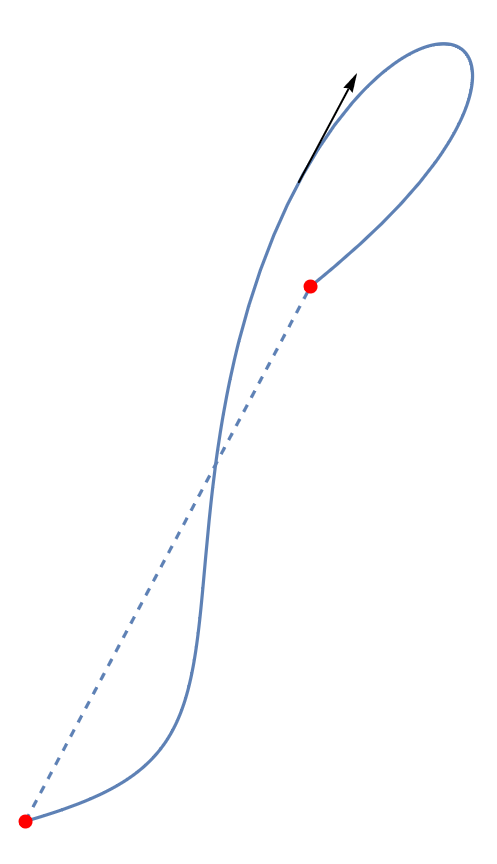
\includegraphics[width=.2\textwidth]{5 The Derivative/Exercise 5.3.4/Exercise 5.3.4 (b).png}
        \caption{\Ex{4} (b) \label{fig:Ex_3_4_b}}
    \end{figure}
    An illustration of this result is shown in figure \ref{fig:Ex_3_4_b}.
\end{enumerate}

\ex{5}
\begin{proof}
    Let $h(x)=f(x)-x$ then we are trying to find where 
    $h(x)$ is zero. Now since $f'(x)\neq 1$ then 
    $h'(x) = f'(x)-1 \neq 0$. For any $x,y \in [a,b]$ with 
    $x<y$
    \begin{align*}
        \frac{h(y)-h(x)}{y-x} = h'(c) \neq 0
    \end{align*}
    for some $c \in (x,y)$ which implies $h(y) \neq h(x)$ for 
    $x\neq y$. Suppose there is one fixed point at $d \in [a,b]$,
    then $h(d)=0$ and $0=h(d)\neq h(y)$ so there are no more fixed 
    points.
\end{proof}

\ex{6}
\begin{proof}
    Let's define $h(x)=g(x)-x$, then in terms of
    $h$ we need to show $h(d) \Leftrightarrow h'(1)>0$. 

    The conditions assumed on $g$ translate to $h$ as:
    \begin{gather*}
        h(0)>0 \\
        h(1) = g(1)-1=0 \\
        h''(x) > 0
    \end{gather*}

    $(\Rightarrow)$ Suppose $h(d)=0$ for som e$d\in (0,1)$, then 
    $h''$ positive implies $h'$ is strcitly monotonic increasing.
    So if $h(d)=0$ then $h(x)>0$ for $x>d$. Hence $h'(1)>0$.

    $(\Leftarrow)$ Suppose $h'(1)>0$. Now $h(0)>0$ and $h(1)=0$. Since 
    $h'$ is strcitly increasing then $h'(0)<0$. 
    So we have $h'(0)<0$ and $h'(1)>0$ and since $h'$ is continuous then 
    by the IVT there exists $d\in (0,1)$ s.t. $h(d)=0$.
\end{proof}

\ex{7}
\begin{enumerate}[label=(\alph*)]
    \item 
    \begin{proof}
        $(\Rightarrow)$ Suppose $f$ is increasing. 
        Since $f$ is differentiable on $(a,b)$ then 
        \begin{align*}
            f'(c) = \lim_{x\rightarrow c} \frac{f(x)-f(c)}{x-c}
        \end{align*}
        exists for any $c\in (a,b)$.
        Hence, consider sequence $(x_n)\rightarrow c$ where 
        $(x_n)\in (a,b)$ and $x_n<c$ for all $n\in \mathbb{N}$.
        Hence, 
        \begin{align*}
            x_n - c < 0 \Rightarrow f(x_n) f(c) \leq 0
        \end{align*}
        so 
        \begin{align*}
            \frac{f(x_n)-f(c)}{x_n-c} > 0
        \end{align*}
        for all $n\in \mathbb{N}$.
        By the order limit \Thm this implies $f'(c)\geq 0$.
        Since $c$ was arbitrary then $f'(x)\geq 0$ for $x\in(a,b)$.
    
        $(\Leftarrow)$ Suppose $f'(x)\geq 0$ for $x\in (a,b)$.
        For any $x,y\in (a,b)$ s.t. $x<y$ then by the MVT
        \begin{align*}
            f'(c) = \frac{f(y)-f(x)}{y-x} \geq 0
        \end{align*}
        for some $c\in (x,y)$.
        However this implies $f(y)>f(x)$. Since $x,y$ where 
        arbitrary then $f$ is increasing.
    \end{proof}

    \item
    From our previous studies we know $x^2 \sin(1/x)$ is
    differentiable on $\mathbb{R}$. Hence, the derivative of 
    $g$ is given by
    \begin{align*}
        g'(x) = \begin{cases}
            1/2 + 2x \sin(1/x) - \cos(1/x) & x\neq 0 \\
            1/2 & x=0
        \end{cases}
    \end{align*}
    To show $g$ is not increasing on any open interval we need to show 
    $g'(x)<0$ for at least a single $x$ in every open interval around zero.
    
    For some interval $(-\varepsilon, \varepsilon)$, assume $\varepsilon<1/8$,
    then $-1/4 \leq 2x\sin(1/x) \leq 1/4$ and $-1 \leq \cos(1/x) \leq 1$ so 
    since $\sin$ and $\cos$ are $\pi/2$ out of phase we know peaks will meet 
    with trophs and vice versa so
    \begin{align*}
        -3/4 \leq 2x\sin(1/x) - \cos(1/x) \leq 3/4
    \end{align*}
    so $g$ is not strcitly increasing since every open interval around zero of
    $g'$ is not strictly non-negative then $g$ is not increasing. 
\end{enumerate}

\ex{8}
\begin{proof}
    Suppose $g'(c)\neq 0$, without loss of generality assume 
    $g'(c)>0$. For $\varepsilon=g'(c)/2$ there exists $\delta>0$
    s.t. 
    \begin{align*}
        0<|x-c|<\delta \Rightarrow |\frac{g(x)-g(c)}{x-c}-g'(c)| < g'(c)/2
    \end{align*}
    This implies 
    \begin{align*}
        0<g'(c)/2 < \frac{g(x)-g(c)}{x-c} < 3g'(c)/2
    \end{align*}
    Multiplying through by $x-c$
    \begin{align*}
        \begin{cases}
            g(x)-g(c) > 0 & x < c \\
            g(x)-g(c) < 0 & x > c
        \end{cases} \\
        \Rightarrow \begin{cases}
            g(x) > g(c) & x < c \\
            g(x) < g(c) & x > c
        \end{cases}
    \end{align*}
    so $g(x)\neq g(c)$ for $c \in V_\delta(c)$ excluding 
    $x=c$ ofcourse.
\end{proof}

\ex{9}
\begin{proof}
    Choose $M>0$,
    since $\lim g(x) = 0$ then there exists $\delta_1>0$ s.t. 
    \begin{align*}
        0<|x-c|<\delta_1 \Rightarrow |g(x) - g(c)| < \frac{L-1}{M}
    \end{align*}
    Since $\lim f(x)=L$ then there exists $\delta_1>0$ s.t. 
    \begin{align*}
        0<|x-c|<\delta_2 \Rightarrow |f(x) - f(c)| < 1 \Rightarrow L-1<f(x)<L+1
    \end{align*}
    so for $\delta=\min\{\delta_1,\delta_2\}$
    \begin{align*}
        0<|x-c|<\delta \Rightarrow |\frac{f(x)}{g(x)}| > |\frac{L-1}{(L-1)/M}| > M
    \end{align*}
    Hence, $f(x)/g(x) \rightarrow \infty$
\end{proof}

\ex{10}
Assume $f$ is bounded by $M$ i.e. $f(x)<M$. Since 
$\lim g(x) = \infty$ then for $\varepsilon>0$ there exists 
$\delta>0$ s.t. 
\begin{align*}
    0<|x-c|<\delta \Rightarrow |g(x)|>\frac{M}{\varepsilon}
\end{align*}
This implies 
\begin{align*}
    |\frac{f(x)}{g(x)}| < \varepsilon
\end{align*}

\ex{11}
\begin{proof}
    $\lim f'(x)/g'(x)=L$ implies that for $\varepsilon>0$ 
    there exists $\delta>0$ s.t. 
    \begin{align*}
        0<|x-a|<\delta \Rightarrow |\frac{f'(x)}{g'(x)}-L|\varepsilon
    \end{align*}
    Since $f,g$ are differentiable on an interval containing $a$ then 
    $f,g$ are differentiable on the interval $[a,x]$ where $a<x<a+\delta$.
    Then by the generalized MVT 
    \begin{align*}
        (f(x)-f(a))g'(c) = (g(x)-g(a))f'(c)
    \end{align*}
    Since $g(a)=f(a)=0$ then 
    \begin{align*}
        f(x)g'(c) = g(x)f'(c)
    \end{align*}
    for some $c\in (a,x)$.
    However, $c,x\in V_\delta(a)$ so 
    \begin{align*}
        \varepsilon>|\frac{f'(c)}{g'(c)}-L|=|\frac{f'(x)}{g'(x)}-L|
    \end{align*}
    Since $x\in V_\delta(a)$ was arbitrary then $|\frac{f'(x)}{g'(x)}-L|<\varepsilon$
    for any $x\in V_\delta(a)$.
\end{proof}

\ex{12}
\begin{proof}
    Since $f',g'$ are continuous as $a$ then 
    \begin{align*}
        \lim_{a\rightarrow a}\frac{f'(x)}{g'(x)} &= \frac{f'(a)}{g'(a)} \\
        &= \frac{\lim_{x\rightarrow a}\frac{f(x)-f(a)}{x-a}}{\lim_{x\rightarrow a}\frac{g(x)-g(a)}{x-a}} \\
        &= \lim_{x\rightarrow a} \frac{\frac{f(x)-f(a)}{x-a}}{\frac{g(x)-g(a)}{x-a}} \\  
        &= \lim_{x\rightarrow a} \frac{f(x)}{g(x)}    
    \end{align*}
\end{proof}

\ex{13}
Since $f,g$ are continuous at $a$ then 
\begin{gather*}
    0=\lim_{x\rightarrow 0} f(x)=  f(\lim_{x\rightarrow 0} x) = f(0) \\
    0=\lim_{x\rightarrow 0} g(x)=  g(\lim_{x\rightarrow 0} x) = g(0)
\end{gather*}
\clearpage

\twocolumn[
  \begin{@twocolumnfalse}
    \section{Sequences and Series of Functions}
  \end{@twocolumnfalse}
]
\setcounter{subsection}{1}
\subsection{Uniform Convergence of a Sequence of Functions}

\ex{1}
\begin{enumerate}[label=(\alph*)]
    \item 
    \begin{align*}
        \lim_n f_n(x) = \lim \frac{x}{\frac{1}{n}+x^2} = \frac{x}{\lim \frac{1}{n}+x^2} = \frac{1}{x}
    \end{align*}

    \item
    The convergence is not uniform since
    \begin{align*}
        |f_x(x)-f(x)| = \frac{1}{nx^3+x}
    \end{align*}
    We require 
    \begin{align*}
        \frac{1}{nx^3+x} < \varepsilon
    \end{align*}
    This occurs when
    \begin{align*}
        n > \frac{1-x\varepsilon}{x^3 \varepsilon}
    \end{align*}
    However, there is no upper bound in dependent of $x$ since as 
    $x$ gets closer to the origin $ \frac{1-x\varepsilon}{x^3 \varepsilon}$
    increases indefinitely.
    
    \item
    $f_n \rightarrow f$ does not converge uniformly on $(0,1)$ since as 
    we mentioned in (a) values near the origin are problematic.

    \item
    $f_n\rightarrow f$ uniformly on $(1\infty)$ since we require $nx^3+x>\frac{1}{\varepsilon}$
    which is bounded below by 
    \begin{align*}
        nx^2+x > n+1
    \end{align*}
    This implies $|f_n(x)-f(x)|<\varepsilon$ for $n>\frac{1}{\varepsilon}-1$
    for all $x\in (1,\infty)$.
\end{enumerate}

\ex{2}
\begin{align*}
    \lim_n g_n(x) &= \lim_n \frac{x}{2} + \lim_n \frac{\sin(nx)}{2n} \\
                &= \frac{x}{2} + 0 \\
                &= x/2
\end{align*}
The convergence is uniform on $\mathbb{R}$ since for some $\varepsilon>0$
choose $N>\frac{1}{\varepsilon}$ which ensures
\begin{align*}
    |\frac{\sin(nx)}{2x}| \leq \frac{1}{2n} < \varepsilon/2 < \varepsilon
\end{align*}

\ex{3}
\begin{enumerate}[label=(\alph*)]
    \item 
    \begin{align*}
        \lim_n h_n(x) = \frac{x}{1+\lim_n x^n}
    \end{align*}
    Then 
    \begin{align*}
        \lim_n h_n(x) = \begin{cases}
            x & x < 1 \\
            \frac{1}{x} & x=1 \\
            0 & x>1
        \end{cases}
    \end{align*}
    since $(x_n)\rightarrow 0$ for $x<1$.

    \item
    Since the limit function is discontinuous and $h_n$ is continuous
    and uniform convergence preserves continuity then the converegence 
    must be pointwise.

    \item

\end{enumerate}


\ex{4}
The solution to $f_n'(c)=0$ is $c=\pm \frac{1}{\sqrt n}$.
The limiting function is given by $f(x)=0$. For some $\varepsilon>0$
we require 
\begin{align*}
    |f_n(x)| < \varepsilon
\end{align*}
It is sufficient to ensure only that 
\begin{align*}
    |f_n(\frac{1}{\sqrt n})| < \varepsilon
\end{align*}
This implies $n>\frac{1}{4\varepsilon^2}$.

\ex{5}
\begin{enumerate}[label=(\alph*)]
    \item 
    It is not difficult to see 
    \begin{align*}
        \lim_n f_n(x) = \begin{cases}
            0 & x=0 \\
            1 & x\neq 0
        \end{cases}
    \end{align*}
    The convergence is not uniform since $f_n$ are continuous by 
    $f$ is discontinuous.

    \item
    Consider,
    \begin{align*}
        f_n(x) = \frac{n x}{1+n x^2}
    \end{align*}
    However 
    \begin{align*}
        f(x) = \begin{cases}
            0 & x=0 \\
            \frac{1}{x} & x \neq 0
        \end{cases}
    \end{align*}
\end{enumerate}

\ex{6}
\begin{proof}
    $(\Rightarrow)$ Suppose $(f_n)$ converges uniformly, then 
    for $\varepsilon>0$ there
    exists $N\in \mathbb{N}$ s.t. 
    \begin{align*}
        |f_n(x)-f(x)| < \varepsilon/2
    \end{align*}
    for $n\geq N$. Hence, for $n>m/geq N$
    \begin{align*}
        |f_n(x)-f_m(x)| &\leq |f_n(x) - f(x)| + |f_m(x) - f(x)| \\
                        &< \varepsilon/2 + \varepsilon/2 \\
                        &= \varepsilon 
    \end{align*}

    $(\Leftarrow)$ Suppose there exists $N$ s.t. for all $x\in A$
    \begin{align*}
        |f_n(x)-f_m(x)| < \varepsilon/2
    \end{align*} 
    for $n>m\geq N$.

    Now $(f_n(x))$ is a cauchy sequence for all $x\in A$ so the sequence is 
    convergent so let $(f_x(x))\rightarrow f(x)$ for all $x\in A$.

    Now since the absolute value function is continuous then 
    \begin{align*}
        \lim_n |f_m(x)-f_n(x)| = |f_m(x)-\lim_n f_n(x)| = |f_m(x)-f_n(x)| \leq \varepsilon/2
    \end{align*}
    for $m\geq N$.

    Hence,
    \begin{align*}
        |f_n(x) - f(x)| & \leq |f_n(x)-f_m(x)| + |f_m(x)-f(x)| \\
                        &\leq \varepsilon/2 + \varepsilon/2 \\
                        &= \varepsilon
    \end{align*}
    for $n\geq N$. Implicit is the assumption that 
    $m\geq N$. The first inequailty follows since we assumed $f_n$
\end{proof}

\ex{7}
\begin{proof}
    Since $f_n \rightarrow f$ uniformly choose $N \in \mathbb{N}$
    s.t. 
    \begin{gather*}
        |f(x)-f_N(x)| < \varepsilon/3 \\
    \end{gather*}
    for all $x$.
    Next choose $\delta>0$ s.t. 
    \begin{align*}
        |x-y|< \delta \Rightarrow |f_N(x)-f_N(y)|<\varepsilon/3
    \end{align*}
    Then 
    \begin{align*}
        |f(x)-f(y)| &\leq |f(x)-f_N(x)| + |f_N(x)-f_N(y)| + |f(x)-f(y)| \\
        &< \varepsilon/3 + \varepsilon/3 + \varepsilon/3 \\
        &= \varepsilon
    \end{align*}
    for $|x-y|< \delta$.
\end{proof}

\ex{8}
\begin{enumerate}[label=(\alph*)]
    \item 
    False, consider compact set $[-5,5]$ where 
    \begin{align*}
        f_n(x) = \frac{nx}{1+nx^2}
    \end{align*}
    which converges to 
    \begin{align*}
        f(x) = \begin{cases}
            0 & x=0 \\
            1/x & x\neq 0
        \end{cases}
    \end{align*}
    However, the convergence is not uniform since $f_n$
    is continuous but $f$ is discontinuous.

    \item
    \begin{proof}
        Suppose $f_n \rightarrow f$ uniformly and 
        $g(x)<M$, then there exists 
        $N\in \mathbb{N}$ s.t. 
        \begin{align*}
            |f_n(x)-f(x)| < \frac{\varepsilon}{M}
        \end{align*}
        We hypothesise that $f_n g \rightarrow fg$:
        \begin{align*}
            |f_n(x)g(x)-f(x)g(x)| &= |g(x)| |f_n(x)-f(x)| \\
                                &< M |f_n(x)-f(x)| \\
                                &< \varepsilon
        \end{align*}
    \end{proof}

    \item
    \begin{proof}
        \begin{align*}
            |f(x)| &\leq |f(x)-f_n(x)| + |f_n(x)|
        \end{align*}
        Since $f_n \rightarrow f$ uniformly then we may choose 
        $N$ s.t.
        \begin{align*}
            |f(x)-f_n(x)| < \varepsilon
        \end{align*}
        for $n\geq N$. Also, we assumed $f_n < M$ so 
        \begin{align*}
            |f(x)| &\leq \varepsilon + M
        \end{align*}
    \end{proof}

    \item
    \begin{proof}
        Since $f_n\rightarrow f$ uniformly on $A,B$ then 
        there exist $N_1, N_2$ s.t. 
        \begin{gather*}
            |f(x)-f_{n_1}(x)| < \varepsilon \quad n_1\geq N_1 \\
            |f(x)-f_{n_2}(x)| < \varepsilon \quad n_2\geq N_2
        \end{gather*}
        Let $N=\max\{N_1, N_2\}$ then 
        \begin{align*}
            |f(x)-f_{n}(x)| < \varepsilon \quad n_\geq N
        \end{align*}
        on $A\cup B$.
    \end{proof}

    \item
    \begin{proof}
        Suppose $f_n$ is increasing but $f$ is not. Since $f$
        is not increasing then there exist $x,y$ s.t. $x<y$
        but $f(x)>f(y)$. Since $f_n$ converges uniformly then 
        there exists $N$ s.t. 
        \begin{align*}
            |f(x)-f_{n}(x)| < \varepsilon = |f(x)-f(y)|/3 \\
            |f(y)-f_{y}(x)| < \varepsilon = |f(x)-f(y)|/3
        \end{align*}
        for $n\geq N$. This implies 
        \begin{gather*}
            f(x)-\varepsilon < f_n(x) < f(x)+\varepsilon \\
            f(y)-\varepsilon < f_n(y) < f(y)+\varepsilon
        \end{gather*}
        Hence, 
        \begin{align*}
            f_n(y) < f(y)+\varepsilon < f(x)-\varepsilon<f_n(x)
        \end{align*}
        which is a contradiction since we assumed $f_n$ are 
        increasing.
    \end{proof}

    \item
    \begin{proof}
        As it turns out we do not require uniform continuity. 
        We can see this using a different proof.
        Since $f_n(x)\leq f_n(y)$ for $x<y$ then taking the 
        limit on both sides we obtain 
        \begin{align*}
            \lim_n f_n(x) &\leq \lim_n f_n(y) \\
            f(x) &\leq f(y)
        \end{align*}
    \end{proof}
\end{enumerate}

\ex{9}
\begin{proof}
    Since $g$ is continuous on a compact set then by the extreme 
    value \Thm there exist $x_0,x_1\in K$ s.t. $g(x_0) 
    \leq g(x) \leq g(x_1)$. This implies $1/g(x_1) 
    \leq 1/g(x) \leq g(x_0)$. Hence, $1/g$ is bounded on $K$. This 
    then reduces to \Ex{6.2.8} (b).
\end{proof}

\ex{10}
\begin{proof}
    First we check that the limit exists 
    \begin{align*}
        \lim_n f_n(x) = \lim f(x+1/n) = f(x+\lim 1/n) = f(x)
    \end{align*}

    Now since $f$ is uniformly continuous then we expect that 
    there exists $\delta$ s.t. 
    \begin{align*}
        |x-y| < \delta \Rightarrow |f(x) - f(y)|<\varepsilon
    \end{align*}
    In particular choose $y=x+1/n$, then $|x-y|=1/n$. So choose 
    $N>1/\delta$ so that $|x-y|<\delta$ for $n\geq N$ which 
    implies $|f(x)-f(x+1/n)|<\varepsilon$ so $f_n$ is uniformly
    convergent. 
\end{proof}

As a counter example if $f$ is only assumed continuous, 
consider $f(x)=x^2$ then 
\begin{align*}
    |f_n(x) - f(x)| &= |(x+1/n)^2 - x^2| \\
    &= |\frac{2x}{n}+\frac{1}{n^2}|
\end{align*}
We require this result to be less than $\varepsilon$ which 
occurs when $n>\frac{x+\sqrt{x+\varepsilon}}{\varepsilon}$
which cannot be made independent of $x$.

\ex{11}
\begin{enumerate}[label=(\alph*)]
    \item 
    \begin{proof}
        We claim $(f_n+g_n)\rightarrow (f+g)$.
        Now
        \begin{align*}
            |f(x)-g(x) - f_n(x)-g_n(x)| &\leq |g_n(x)-g(x)| +|g_n(x)-g(x)| 
        \end{align*}
        Since $f_n$ and $g_n$ are uniformly convergent then for some 
        $\varepsilon>0$ there 
        exist $N_1, N_2 \in \mathbb{N}$ s.t. 
        \begin{align*}
            |f_{n_1}(x)-f(x)| < \varepsilon/2 \quad n_1\geq N_1 \\
            |g_{n_2}(x)-g(x)| < \varepsilon/2 \quad n_2\geq N_2
        \end{align*}
        If we choose $N=\max\{N_1, N_2\}$ then 
        \begin{align*}
            |f(x)-g(x) - f_n(x)-g_n(x)| &< \varepsilon/2 + \varepsilon/2 \\
            &= \varepsilon
        \end{align*}
    \end{proof}

    \item
    Consider $f_n(x)=g_n(x)=x+1/n$.

    \item
    \begin{proof}
        Now 
        \begin{align*}
            &|f_n(x)g_n(x)-f(x)g(x)| \\ &= |f_n(x)g_n(x)-f_m(x)g_n(x)+f_m(x)g_n(x)-f_m(x)g_m(x)| \\
            &\leq  |f_n(x)g_n(x)-f_m(x)g_n(x)|+|f_m(x)g_n(x)-f_m(x)g_m(x)| \\
            &=  |f_n(x)-f_m(x)||g_n(x)|+|g_n(x)-g_m(x)||f_m(x)| \\
            &\leq  |f_n(x)-f_m(x)|M+|g_n(x)-g_m(x)|M
        \end{align*}
        By the cauchy criterion we now there exists $N$ s.t. 
        $n>m\geq N$ implies $|f_n(x)-f_m(x)|<\varepsilon/(2M)$ and 
        $|g_n(x)-g_m(x)|<\varepsilon/(2M)$ which implies 
        $|f_n(x)g_n(x)-f(x)g(x)|<\varepsilon$ as required.
    \end{proof}
\end{enumerate}

\ex{12}
\begin{enumerate}[label=(\alph*)]
    \item 
    Assume $g_n \rightarrow 0$ pointwise
    on a compact set $K$ and assume that for each $x\in K$ the sequence $g_n(x)$
    is decreasing. Then if $g_n$ are continuous on $K$,
    then the convergence is uniform.

    \item
    \begin{proof}
        First we prove $K_n$ is comapct:
        \begin{itemize}
            \item $K_n\subseteq K$ which is bounded so $K_n$ is bonuded.
            \item $K_n$ is closed since for any convergent sequence $(x_n)\in K_n$
            which converges to $x$
            \begin{align*}
                g_n(x_n)\geq \varepsilon \Rightarrow \lim g_n(x_n) \geq \varepsilon
            \end{align*}
            Since $g$ is continuous then $ \lim g_n(x_n) = g_n(\lim x_n)=g(x)\geq \varepsilon$
            so $x\in K_n$ and $K_n$ is closed.
        \end{itemize}
        Hence, $K_n$ is compact.

        Now we argue $\{K_n\}$ are a nested sequence of sets:
        If $x\in K_{n+1}$ then $g_{n+1}(x)\geq \varepsilon$. However, since $(g_n)$
        is decreasing then we expect
        \begin{align*}
            \varepsilon \leq g_{n+1}(x) \leq g_n(x)
        \end{align*}
        which implies $x\in K_n$. So $K_{n+1} \subseteq K_n$.

        We are now ready to argue for uniform convergence:
        We know that there exists $x\in \cap_n K_n$. However, this implies $g_n(x)\geq \varepsilon$
        for all $n$. Taking the limit we find $\lim_n g_n(x)\geq \varepsilon = 0$.
        This implies $\varepsilon=0$ which is a contradiction since we assumed $\varepsilon>0$.

        To resolve this contradiction, the NIP property cannot be applied if the intervals
        are everntually empty. Hence, we conclude there exists $N$ s.t. $K_n=\emptyset$
        for $n\geq N$. Hence, for any arbitrary $\varepsilon>0$ there exists $N$
        s.t. $|g_n(x)| < \varepsilon$ for $n\geq N$ which means $g$ is uniformly convergent.
        However, this immedietly implies $(f_n)$ is uniformly convergent.
    \end{proof}
\end{enumerate}

\ex{13}

\ex{14}
\begin{enumerate}[label=(\alph*)]
    \item 
    $f_n(x_1)$ is bounded so by BW there exists a convergent subsequence 
    $f_{n_k}(x_1)$ which converges. 

    \item
    $f_{1,k}(x_2)$ is bounded so by BW there exists a convergent subsequence 
    $f_{2,k}(x_2)$ which converges. $f_{2,k}(x_2)$ has the property that it converges 
    at $x_1$ and $x_2$ now.

    \item
    Repeating the above process i.e. if $f_{m,k}$ corresponds to the subset of functions 
    which where generated from $f_{m-1,k}$ which ensure $f_{m-1,k}(x_{m-1})$
    converges then we can a nested seqeunce of sequences of functions which we denote 
    by $(f_{m,k})$.

    We can visualize this as is done with in Cantor’s
    diagonalization technique as follows: 
    \[
        \begin{array}{c|ccccc}
            x_1 & f_{1,1} & f_{1,2} & f_{1,3} & f_{1,4} & \cdots \\
            x_2 & f_{2,1} & f_{2,2} & f_{2,3} & f_{2,4} & \cdots \\
            x_3 & f_{3,1} & f_{3,2} & f_{3,3} & f_{3,4} & \cdots \\
            \vdots & \vdots & \vdots & \vdots & \vdots & \ddots
         \end{array}
    \]

    If we make a sequence of functions corresponding to the diagonal functions 
    and name this sequence $(g_n)$ then 
    in the above table then we obtain a sequence which converges at every point in 
    $A$ since $g_n(x_m)$ converges for $n\geq m$.
\end{enumerate}

\ex{15}
\begin{enumerate}[label=(\alph*)]
    \item 
    Every $f_n$ is uniformly confinuous, moreover, we can find a single $\delta$
    which ensures $|f_n(x)-f(x)|<\varepsilon$ for every function in the sequence
    simultaniously.

    \item
    $(g_n)$ is not equicontinuous since $x^n$ gets steeper near unity with increasing $n$
    so a $\delta>0$ which works for $g_n$ must everntually fail for sufficiently large $n$.

    However, observe that $g_n$ are each indefinitely uniformly continuous.
\end{enumerate}

\ex{16}
\begin{proof}
    \begin{enumerate}[label=(\alph*)]
        \item 
        The rationals are countable so we consider some enumeration
        $\{r_1,r_2,...\}$ in $[0,1]$ and apply \Ex{14}.
    
        \item
        For fixed $r_i$ we know $g_n(r_j)$ converges so the 
        sequence is cauchy so there exists $N_i$ s.t. 
        \begin{align*}
            |g_s(r_j)-g_t(r_j)|<\varepsilon/3
        \end{align*}
        for $n\geq N_j$.
        Since ${r_i}$ is a finite set we simply take $N=\max_i\{N_i\}$
        then 
        \begin{align*}
            |g_s(r_i)-g_t(r_i)|<\varepsilon/3
        \end{align*}
        for $n\geq N$ for all $1 \leq i \leq m$.
    
        \item
        For arbitrary $x\in[0,1]$ choose $i$ s.t. $x\in V_\delta(r_i)$.
        By construction we know $|x-r_i|<\delta$ so 
        \begin{align*}
            |g_k(r_i)-g_k(x)| < \varepsilon/3
        \end{align*}
        for all $k$. 
        Now
        \begin{gather*}
            |g_s(x)-g_s(r_i)| < \varepsilon/3 \\
            |g_s(x)-g_s(r_i)| < \varepsilon/3
        \end{gather*}
        by equicontinuity.
        \begin{align*}
            |g_t(r_i)-g_t(x)| < \varepsilon/3
        \end{align*}
        for $s,t\geq N$ by (b).
        Hence, 
        \begin{align*}
            |g_s(x)-g_t(x)| &\leq |g_s(x)-g_s(r_i)|+|g_s(r_i)-g_r(r_i)|+|g_t(r_i)-g_t(x)| \\
            &< \varepsilon
        \end{align*}
    \end{enumerate}
\end{proof}
% Ex 6.2.13
\clearpage
\subsection{Uniform Convergence and Differentiation}

\ex{1}
\begin{enumerate}[label=(\alph*)]
    \item 
    Observe, for $N>1/\varepsilon$
    \begin{align*}
        |h_n(x)| &\leq \frac{1}{n} \\
                &< \varepsilon
    \end{align*}
    for $n\geq N$. Since this applies for all $x$ i.e. 
    $N$ is not a function of $x$ then 
    $h_n \rightarrow 0$ uniformly.

    Now
    \begin{align*}
        h'_n(x) = \cos(n x)
    \end{align*}
    As $n$ increases the oscillations increase. However, 
    they increase in multiples of the fundamental angular frequency
    $2\pi$. So $h_n$ converges for $x=2\pi m$ for $m\in \mathbb{N}$.
    
    \item
    We want the amplitude of the oscillations to get smaller with $n$
    however when we differentiate we want the oscillations to grow
    indefinitely.
    This is achieved using 
    \begin{align*}
        h_n(x) = \frac{\sin(nx)}{\sqrt{n}}
    \end{align*}
    Then
    \begin{align*}
        h_n'(x) = \sqrt{n}\cos(nx)
    \end{align*}
    Notice, we didn't need to use squareroot.
\end{enumerate}

\ex{2}
\begin{enumerate}[label=(\alph*)]
    \item 
    Since $|x^n/n|\leq 1/n$ then for $N>1/\varepsilon$
    \begin{align*}
        |g_n(x)| &\leq \frac{1}{n} \\
                &< \varepsilon
    \end{align*}
    for $n\geq N$. Since this applies for all $x$ i.e. 
    $N$ is not a function of $x$ then 
    $g_n \rightarrow g = 0$ uniformly. Clearly $g$ is
    differentiable and $g'(x)=0$.

    \item
    Now 
    \begin{align*}
        g_n'(x) = x^{n-1}
    \end{align*}
    This is the same as studying $(x^n)\rightarrow h$. Then 
    \begin{align*}
        h(x) = \begin{cases}
            0 & x \neq 1 \\
            1 & x = 1
        \end{cases}
    \end{align*}
    The convergence cannot be uniform since $g'_n$ is continuous 
    but $g'$ is discontinuous.
    
    Since the convergence is not uniform we see as 
    expected $h\neq g'$.
\end{enumerate}

\ex{3}
We know $\lim f_n(x)=0$.
Now 
\begin{align*}
    f'_n(x) = \frac{1-nx^2}{(1+nx^2)^2}
\end{align*}
We need to find all the points where the convergence of $f'_n(x)\rightarrow 0$.
Observe for $x=0$ the sequence converges to $0$. For $x\neq 0$
\begin{align*}
    \lim_n \frac{nx^2-1}{n^2 x^4+2nx^2+1} &= \lim_n \frac{\frac{x^2}{n}-\frac{1}{n^2}}{x^2+\frac{2x^2}{n}+\frac{1}{n^2}} \\
    &= \frac{0 - 0}{x^4+0+0} \\
    &= 0
\end{align*}
so $f'(x)=\lim_n f_n'(x)$ for $x\neq 0$.

\ex{4}
\begin{enumerate}[label=(\alph*)]
    \item 
    Now 
    \begin{align*}
        \lim_n g_n(x) = \frac{nx+x^2}{2n} \\
        &= \frac{x+\frac{x^2}{n}}{2} \\
        &= \frac{x}{2}
    \end{align*}
    Hence, $g'(x)=1/2$.

    \item
    Now
    \begin{align*}
        g_n'(x) = \frac{1}{2} + \frac{x}{n}
    \end{align*}
    For interval $[-M,M]$ and $\varepsilon$ choose $N>\frac{M}{\varepsilon}$
    which ensures
    \begin{align*}
        |x/n| \leq M/n < \varepsilon
    \end{align*}
    for all $x\in [-M,M]$. Hence $g'_n$ converges uniformly. 
    Hence, we know $\lim g'_n = g'$. So $g'(x)=1/2$.

    \item

\end{enumerate}

\ex{5}
\begin{proof}
    Fix $x\in [a,b]$ and observe
    \begin{align*}
        |f_n(x) - f_m(x)| \leq |(f_n(x) - f_m(x)) - (f_n(x_0) - f_m(x_0))| + |f_n(x_0) - f_m(x_0)|
    \end{align*}
    Since $f_n(x_0)$ converges then there exists $N_1$ s.t. 
    \begin{align*}
        |f_n(x_0) - f_m(x_0)| < \varepsilon/2
    \end{align*}
    for $n>m\geq N_1$.

    Since $f_n-f_m$ is differentiable then it is continuous so 
    there exists $\alpha \in (x_0,x)$ (or $(x,x_0)$ if $x<x_0$) s.t. 
    \begin{align*}
        f_n'(\alpha) - f_m'(\alpha) = \frac{f_n'(x) - f_m'(x_0) + g_n'(x) - g_m'(x_0)}{x-x_0}|
    \end{align*}
    Now $f_n'$ converges uniformly so there exists $N_2$ s.t. 
    \begin{align*}
        |f_n'(\alpha) - f_m'(\alpha)| < \frac{\varepsilon}{2|x-x_0|}
    \end{align*}
    for $n>m\geq N_2$.

    This implies
    \begin{align*}
        |f_n'(x) - f_m'(x_0) + g_n'(x) - g_m'(x_0)| < \varepsilon/2
    \end{align*}
    Choose $N=\max\{N_1,N_2\}$ which implies 
    \begin{align*}
        |f_n(x) - f_m(x)| < \varepsilon
    \end{align*}
    Since $x$ was chosen arbitrarily then $f_n$ converges uniformly.
\end{proof}
% Ex 6.3.4 (c)
\clearpage
\subsection{Series of Functions}

\ex{1}
\begin{proof}
    Since $\sum g_n$ converges uniformly then the partial sums converge uniformly
    so by the cauchy criterion there exists $N$ s.t. for all $x$
    \begin{align*}
        |g_n(x) + \hdots + g_{m+1}(x)| < \varepsilon
    \end{align*}
    for $n>m\geq N$. Specifically choose $n=m+1$ then 
    \begin{align*}
        |g_n(x)| < \varepsilon
    \end{align*}
    for $n\geq N$. Hence, $g_n \rightarrow 0$ uniformly.
\end{proof}

\ex{2}
\begin{proof}
    Observe
    \begin{align*}
        |f_n(x) + \hdots + f_{m+1}(x)| &\leq  |f_n(x)| + \hdots + |f_{m+1}(x)|  \\
                                    &\leq |M_n| + \hdots + |M_{m+1}|
    \end{align*}
    Since $\sum M_n$ converges absolutely, then there exists $N$ s.t. 
    \begin{align*}
        |M_n| + \hdots + |M_{m+1}| < \varepsilon
    \end{align*} 
    for $n>m\geq N$. This implies
    \begin{align*}
        |f_n(x) + \hdots + f_{m+1}(x)| < \varepsilon
    \end{align*}
    for $n>m\geq N$. Since this is independent of $x$ then the convergence 
    is uniform.
\end{proof}

\ex{3}
\begin{enumerate}[label=(\alph*)]
    \item 
    \begin{proof}
        Since $|\cos(2^n x)/2^n|\leq 1/2^n$ and $\sum  1/2^n$
        converges then by the M-test $\sum \cos(2^n x)/2^n$ converges 
        uniformly. Since each term in the series is continuous and 
        uniform convergence preserves continuity then $g$ is also 
        continuous.
    \end{proof}

    \item
    \begin{proof}
        Since $|x^n/n^2|\leq 1/n^2$ on $[-1,1]$ and $\sum  1/n^2$
        converges then by the M-test $\sum x^n/n^2$ converges 
        uniformly on $[-1,1]$ . Since each term in the series is continuous and 
        uniform convergence preserves continuity then $h$ is also 
        continuous on $[-1,1]$.
    \end{proof}
\end{enumerate}

\ex{4}
\begin{proof}
    Since $|h(2^n x)/2^n|\leq 1/2^n$ and $\sum  1/2^n$
    converges then by the M-test $\sum h(2^n x)/2^n$ converges 
    uniformly. Since each term in the series is continuous and 
    uniform convergence preserves continuity then $g$ is also 
    continuous.
\end{proof}

\ex{5}
\begin{enumerate}[label=(\alph*)]
    \item 
    \begin{proof}
        Let $f_n(x) = \frac{\sin(kx)}{k^3}$, then $f'_n(x) = \cos(kx)/k^2$.
        Now $|\cos(kx)/k^2|\leq 1/k^2$ and $\sum  1/k^2$
        converges then by the M-test $\sum f_n'(x)$ converges 
        uniformly. Observe,
        \begin{align*}
            \sum \sin(0)/k^3 = 0
        \end{align*}
        So we have found at least one convergent point which implies
        $\sum f_n'(x) \rightarrow f'(x)$. Hence, $f$ is differentiable.
        Furthermore, $f'$ is continuous since $\sum f_n'(x)$ converges 
        uniformly.
    \end{proof}

    \item
    Not easily apparently.
\end{enumerate}

\ex{6}
\begin{proof}
    Fix $x_0$ and study the convergence 
    on the interval $[0,x_0]$ using the M-test.
    Now $x^n \leq x_0^n/n<x_0^n$.
    Now $\sum x_0^n$ is a geometric sequence which 
    converges so $\sum x_0^n$ converges 
    uniformly on $[0,x_0]$. Since $x_0$ was arbitrary then
    the convergence is uniform on $[0,1)$.

    Now each term of the series is continuous so 
    the limiting function $f$ is continuous on $[0,1)$.
\end{proof}

\ex{7}
\begin{enumerate}[label=(\alph*)]
    \item 
    \begin{proof}
        Since $|\frac{1}{x^2+n^2}|\leq 1/n^2$ and $\sum  1/n^2$
        converges then by the M-test $\sum \frac{1}{x^2+n^2}$ converges 
        uniformly. Since each term in the series is continuous and 
        uniform convergence preserves continuity then $h$ is also 
        continuous.
    \end{proof}

    \item
    \begin{proof}
        Let $h_n(x) = \frac{1}{x^2+n^2}$, then $h'_n(x) =\frac{-2x}{n^4+x^4+2n^2x^2}$.
        Now $|h'_n(x)|$ peaks at $\pm n/ \sqrt 3$ so $h'_n(x)\leq \frac{3\sqrt 3}{8n^2}$
         and $\sum \frac{3\sqrt 3}{8n^2}$
        converges then by the M-test $\sum g_n'(x)$ converges 
        uniformly. We already know $h_n$ converges on $\mathbb{R}$ from (a)
        so we have found at least one convergent point which implies
        $\sum h_n'(x) \rightarrow h'(x)$. Hence, $h$ is differentiable.
        Furthermore, $h'$ is continuous since $\sum h_n'(x)$ converges 
        uniformly.
    \end{proof}
\end{enumerate}

\ex{8}
\begin{proof}
    Since $|u_n(x)|\leq 1/2^n$ and $\sum  1/2^n$
    converges then by the M-test $\sum u_n(x)$ converges 
    uniformly. Since each term in the series is continuous at irrational points
     and uniform convergence preserves continuity then $h$ is also 
    continuous at irrational points.

    To show $h$ is a monotone function, 
    it is sufficient to show that the partial sums are monotone functions.
    We prove this via induction:
    \begin{itemize}
        \item Base case: $s_1(x) = u_1(x)$ which is monotone increasing.
        \item Induction on $n$: $u_n$ is increasing then adding $u_{n+1}$ must 
        also be increasing since for $x<y$, $s_{n+1}(x) = s_{n}(x)+u_{n+1}(x) 
        \leq s_{n}(y)+u_{n+1}(y) = s_{n+1}(y)$
    \end{itemize}
    so $s_n$ is monotone increasing by the induction hypothesis.
    So by the order limit \Thm this implies 
    \begin{gather*}
        \lim_n s_n(x) \leq \lim_n s_n(y) \\
        h(x) \leq h(y)
    \end{gather*}
\end{proof}
\clearpage

\end{document}
